%% ============================================================
%% NAS-PINN Thesis Defense — Professional Beamer Presentation
%% Compile on Overleaf with Figures/ folder uploaded
%% ============================================================
\documentclass[aspectratio=169, 11pt]{beamer}

% ── Custom minimal theme ─────────────────────────────────────
\usetheme{default}
\usecolortheme{default}

% Colours
\definecolor{primary}{RGB}{26,74,92}      % dark teal
\definecolor{accent}{RGB}{31,115,158}     % mid blue
\definecolor{lightbg}{RGB}{245,248,250}   % very light
\definecolor{textgray}{RGB}{80,80,80}
\definecolor{ruled}{RGB}{200,215,222}

% Remove all navigation junk
\setbeamertemplate{navigation symbols}{}
\setbeamertemplate{headline}{}

% Frame title — thin teal bar, white text
\setbeamertemplate{frametitle}{%
  \vskip-2pt
  \begin{beamercolorbox}[wd=\paperwidth, ht=2.2em, dp=0.6em, leftskip=0.8em]{frametitle}
    \usebeamerfont{frametitle}\insertframetitle
    \ifx\insertframesubtitle\empty\else
      \par\vskip-2pt
      {\usebeamerfont{framesubtitle}\color{ruled}\insertframesubtitle}
    \fi
  \end{beamercolorbox}%
  \vskip-1pt
  \textcolor{ruled}{\rule{\paperwidth}{0.4pt}}%
}

% Footer — minimal
\setbeamertemplate{footline}{%
  \vskip2pt
  \hbox{\hspace{0.8em}%
    \textcolor{textgray}{\tiny\insertshortauthor\hfill
    \insertshorttitle\hfill
    \insertframenumber\,/\,\inserttotalframenumber}%
  \hspace{0.8em}}%
  \vskip4pt
}

% Colours
\setbeamercolor{frametitle}{fg=white, bg=primary}
\setbeamercolor{title}{fg=white}
\setbeamercolor{subtitle}{fg=ruled}
\setbeamercolor{structure}{fg=accent}
\setbeamercolor{block title}{fg=white, bg=accent}
\setbeamercolor{block body}{bg=lightbg}
\setbeamercolor{alerted text}{fg=accent}

% Fonts
\setbeamerfont{frametitle}{size=\large, series=\bfseries}
\setbeamerfont{title}{size=\huge, series=\bfseries}
\setbeamerfont{subtitle}{size=\normalsize}
\setbeamerfont{block title}{size=\normalsize, series=\bfseries}
\setbeamerfont{block body}{size=\small}

% Bullet style
\setbeamertemplate{itemize item}{\color{accent}\textbullet}
\setbeamertemplate{itemize subitem}{\color{accent}--}
\setbeamertemplate{enumerate item}{\color{accent}\insertenumlabel.}

% ── Packages ─────────────────────────────────────────────────
\usepackage[utf8]{inputenc}
\usepackage[T1]{fontenc}
\usepackage{lmodern}
\usepackage{graphicx}
\graphicspath{{Figures/}{Figures/seed_results/}}
\usepackage{booktabs}
\usepackage{amsmath,amssymb}
\usepackage{tikz}
\usepackage{xcolor}
\usepackage{colortbl}
\usepackage{microtype}

% ── Section slide helper ─────────────────────────────────────
\newcommand{\sectionslide}[2]{%
  \begin{frame}[plain]
    \begin{tikzpicture}[remember picture, overlay]
      \fill[primary] (current page.south west) rectangle (current page.north east);
      \node[anchor=center, text=white] at (current page.center)
        {\fontsize{32}{40}\bfseries #1};
      \node[anchor=center, text=ruled, yshift=-1.6cm] at (current page.center)
        {\large #2};
    \end{tikzpicture}
  \end{frame}
}

% ── Metadata ─────────────────────────────────────────────────
\title[NAS-PINN Thesis Defense]{%
  NAS-Guided FEM-Anchored PINNs\\[4pt]
  for Transient Heat Transfer Simulation}
\subtitle{Multi-Step Window Prediction for Industrial Water Quenching\\
  of A356 Aluminium Automotive Subframes}
\author[O.\ Cetinkaya]{Omer Cetinkaya\\[4pt]
  {\small Supervisor: Prof.\ Turgay Celik}}
\institute{University of Agder (UiA), Norway}
\date{June 2026}

% ============================================================
\begin{document}
% ============================================================

%% ── TITLE ───────────────────────────────────────────────────
\begin{frame}[plain]
  \begin{tikzpicture}[remember picture, overlay]
    \fill[primary] (current page.south west) rectangle (current page.north east);
    % White panel
    \fill[white] ([yshift=-1.8cm]current page.north west)
                 rectangle ([yshift=2.0cm]current page.south east);
    % Title
    \node[anchor=center, text=white, yshift=2.6cm]
      at (current page.center)
      {\fontsize{26}{32}\bfseries NAS-Guided FEM-Anchored PINNs};
    \node[anchor=center, text=ruled, yshift=1.8cm]
      at (current page.center)
      {\fontsize{16}{20}\selectfont for Transient Heat Transfer Simulation};
    % Subtitle white panel
    \node[anchor=center, text=primary, yshift=0.6cm]
      at (current page.center)
      {\fontsize{12}{16}\itshape
        Multi-Step Window Prediction for Industrial Water Quenching\\[2pt]
        of A356 Aluminium Automotive Subframes};
    % Author
    \node[anchor=center, text=primary, yshift=-0.6cm]
      at (current page.center)
      {\fontsize{13}{18}\bfseries Omer Cetinkaya};
    \node[anchor=center, text=textgray, yshift=-1.15cm]
      at (current page.center)
      {\fontsize{10}{14}\selectfont
        Supervisor: Prof.\ Turgay Celik \quad|\quad
        University of Agder \quad|\quad 2026};
    % Bottom bar
    \fill[accent] ([yshift=0.9cm]current page.south west)
                  rectangle ([yshift=0.3cm]current page.south east);
    \node[anchor=center, text=white, yshift=0.6cm]
      at (current page.south)
      {\small Thesis Defense \quad|\quad June 2026};
  \end{tikzpicture}
\end{frame}

%% ── OUTLINE ─────────────────────────────────────────────────
\begin{frame}{Outline}
  \begin{columns}[t]
    \begin{column}{0.48\textwidth}
      \begin{enumerate}\setlength\itemsep{10pt}
        \item \textbf{Introduction}\\
              {\small\color{textgray}
                Motivation $\cdot$ Background $\cdot$ Problem}
        \item \textbf{Methodology}\\
              {\small\color{textgray}
                FEM $\cdot$ NAS-PINN $\cdot$ MSWP $\cdot$ Benchmarks}
        \item \textbf{Results}\\
              {\small\color{textgray}
                2D $\cdot$ Adaptive-$k$ $\cdot$ 3D $\cdot$ Thermal Fin $\cdot$ PINN-only}
      \end{enumerate}
    \end{column}
    \begin{column}{0.48\textwidth}
      \begin{enumerate}\setlength\itemsep{10pt}
        \setcounter{enumi}{3}
        \item \textbf{Discussion}\\
              {\small\color{textgray}
                Cross-domain $\cdot$ Practical guidance}
        \item \textbf{Conclusion}\\
              {\small\color{textgray}
                Summary $\cdot$ Contributions $\cdot$ Future steps}
      \end{enumerate}
      \vspace{1cm}
      \begin{block}{Key Question}
        \small How many FEM solver calls can be replaced
        by PINN predictions while keeping MAE $\leq 15$\,\textdegree C?
      \end{block}
    \end{column}
  \end{columns}
\end{frame}

% ============================================================
\sectionslide{01\quad Introduction}{Motivation $\cdot$ Background $\cdot$ Problem Statement}
% ============================================================

\begin{frame}{Introduction: Why This Problem Matters}
  \begin{columns}[t]
    \begin{column}{0.32\textwidth}
      \begin{block}{The Process}
        \small
        A356 aluminium subframes undergo water quenching after heat
        treatment at 540\,\textdegree C.

        \smallskip
        Non-uniform cooling $\to$ thermal gradients $\to$ distortion.

        \smallskip
        Mortensen et al.\ (2026): rack optimisation reduces distortion
        from $\approx$3\,mm to $\approx$1\,mm.
      \end{block}
    \end{column}
    \begin{column}{0.32\textwidth}
      \begin{block}{The Challenge}
        \small
        Full thermo-mechanical FEM (StaMiSim):
        \begin{itemize}\itemsep1pt
          \item $\approx$3\,M finite elements
          \item 27 coupled domains
          \item $\approx$2\,min per FEM step
        \end{itemize}
        \smallskip
        Design optimisation:\\
        100 runs $\times$ 40\,min $=$ \textbf{67\,hours}
      \end{block}
    \end{column}
    \begin{column}{0.32\textwidth}
      \begin{block}{This Thesis}
        \small
        FEM-anchored NAS-PINN hybrid:
        \begin{itemize}\itemsep1pt
          \item FEM anchors selected steps
          \item NAS-PINN predicts between
          \item Skip factor $k$ controls budget
        \end{itemize}
        \smallskip
        \textbf{Target:} 65--85\% fewer FEM calls,
        MAE $\leq 15$\,\textdegree C
      \end{block}
    \end{column}
  \end{columns}
\end{frame}

\begin{frame}{Background: Building Blocks}
  \begin{columns}[t]
    \begin{column}{0.48\textwidth}
      \textbf{Heat Equation (transient):}
      \[
        \rho c_p\,\frac{\partial T}{\partial t}
        = \nabla\!\cdot\!(k_T\nabla T),
        \quad
        k_T\frac{\partial T}{\partial n} = -h(T-T_w)
      \]
      \smallskip
      \textbf{FEM reference solver:}
      \begin{itemize}
        \item Crank--Nicolson, $\Delta t_\text{int}=0.5$\,s (stable)
        \item Exports field every 1.5\,s $\to$ 21 snapshots
        \item Each snapshot $=$ one FEM solver call
      \end{itemize}
    \end{column}
    \begin{column}{0.48\textwidth}
      \textbf{Physics-Informed Neural Networks:}
      \[
        \mathcal{L} =
        w_\text{pde}\mathcal{L}_\text{pde}
        + w_\text{bc}\mathcal{L}_\text{bc}
        + w_\text{end}\mathcal{L}_\text{end}
      \]
      \begin{itemize}
        \item PDE encoded in loss — no labels needed
        \item Sensitive to architecture choice
      \end{itemize}
      \smallskip
      \textbf{Neural Architecture Search (NAS):}
      \begin{itemize}
        \item Automates depth, width, activation
        \item Run once on rectangle $\to$ deployed everywhere
        \item Three strategies: Bayesian/TPE, NSGA-II, NSGA-III
      \end{itemize}
    \end{column}
  \end{columns}
\end{frame}

\begin{frame}{Problem Statement}
  \begin{center}
    \begin{beamercolorbox}[wd=0.92\textwidth, sep=10pt, center]{block title}
      \large\bfseries
      How many FEM solver calls can be replaced by PINN predictions\\
      without exceeding a temperature error of 15\,\textdegree C?
    \end{beamercolorbox}
  \end{center}
  \vspace{0.4em}
  \begin{columns}[t]
    \begin{column}{0.38\textwidth}
      \centering
      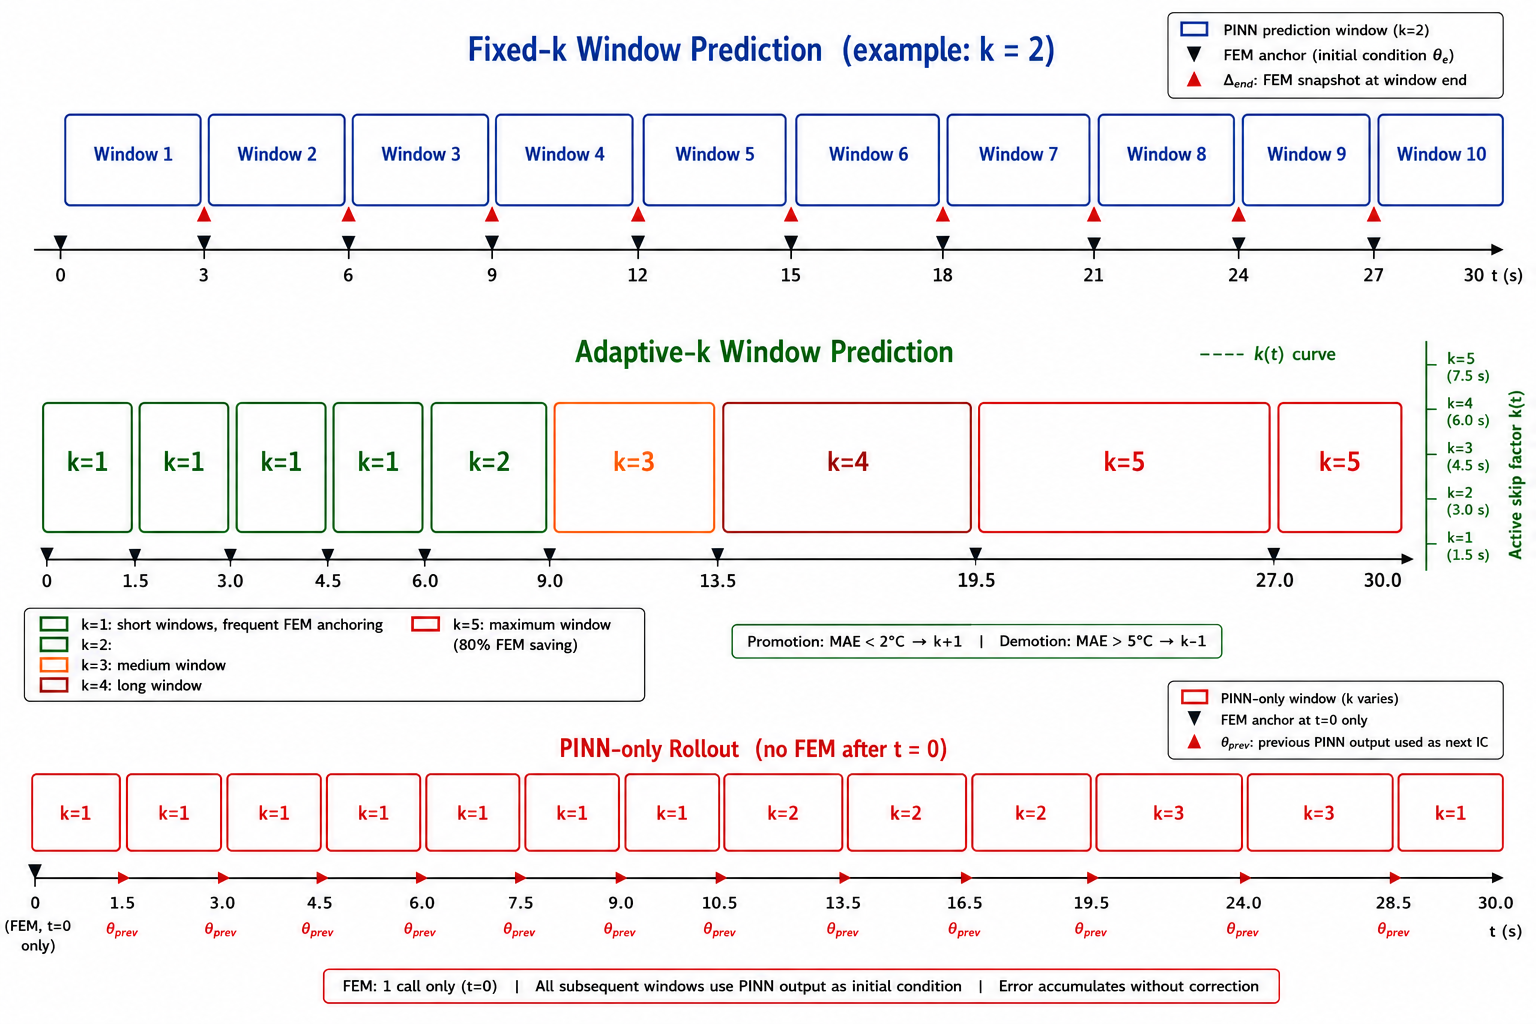
\includegraphics[width=0.95\textwidth]{fig_mswp_three_modes.png}
    \end{column}
    \begin{column}{0.28\textwidth}
      \textbf{Skip factor $k$:}
      \begin{center}\small
      \begin{tabular}{ccc}
        \toprule
        $k$ & Calls & Saving\\
        \midrule
        1 & 20 & 0\%\\
        3 &  7 & 65\%\\
        \rowcolor{lightbg}
        5 &  4 & \textbf{80\%}\\
        \bottomrule
      \end{tabular}
      \end{center}
    \end{column}
    \begin{column}{0.30\textwidth}
      \textbf{Three modes:}
      \begin{enumerate}\itemsep4pt\small
        \item FEM-anchored fixed $k$
        \item FEM-anchored adaptive $k$
        \item PINN-only (stress test)
      \end{enumerate}
      \smallskip
      {\small Tolerance from Mortensen et al.:}\\
      {\small MAE $\leq$ 15\,\textdegree C}
    \end{column}
  \end{columns}
\end{frame}

% ============================================================
\sectionslide{02\quad Methodology}{FEM Solver $\cdot$ NAS-PINN $\cdot$ MSWP $\cdot$ Benchmarks}
% ============================================================

\begin{frame}{Methodology: Framework Overview}
  \begin{columns}
    \begin{column}{0.56\textwidth}
      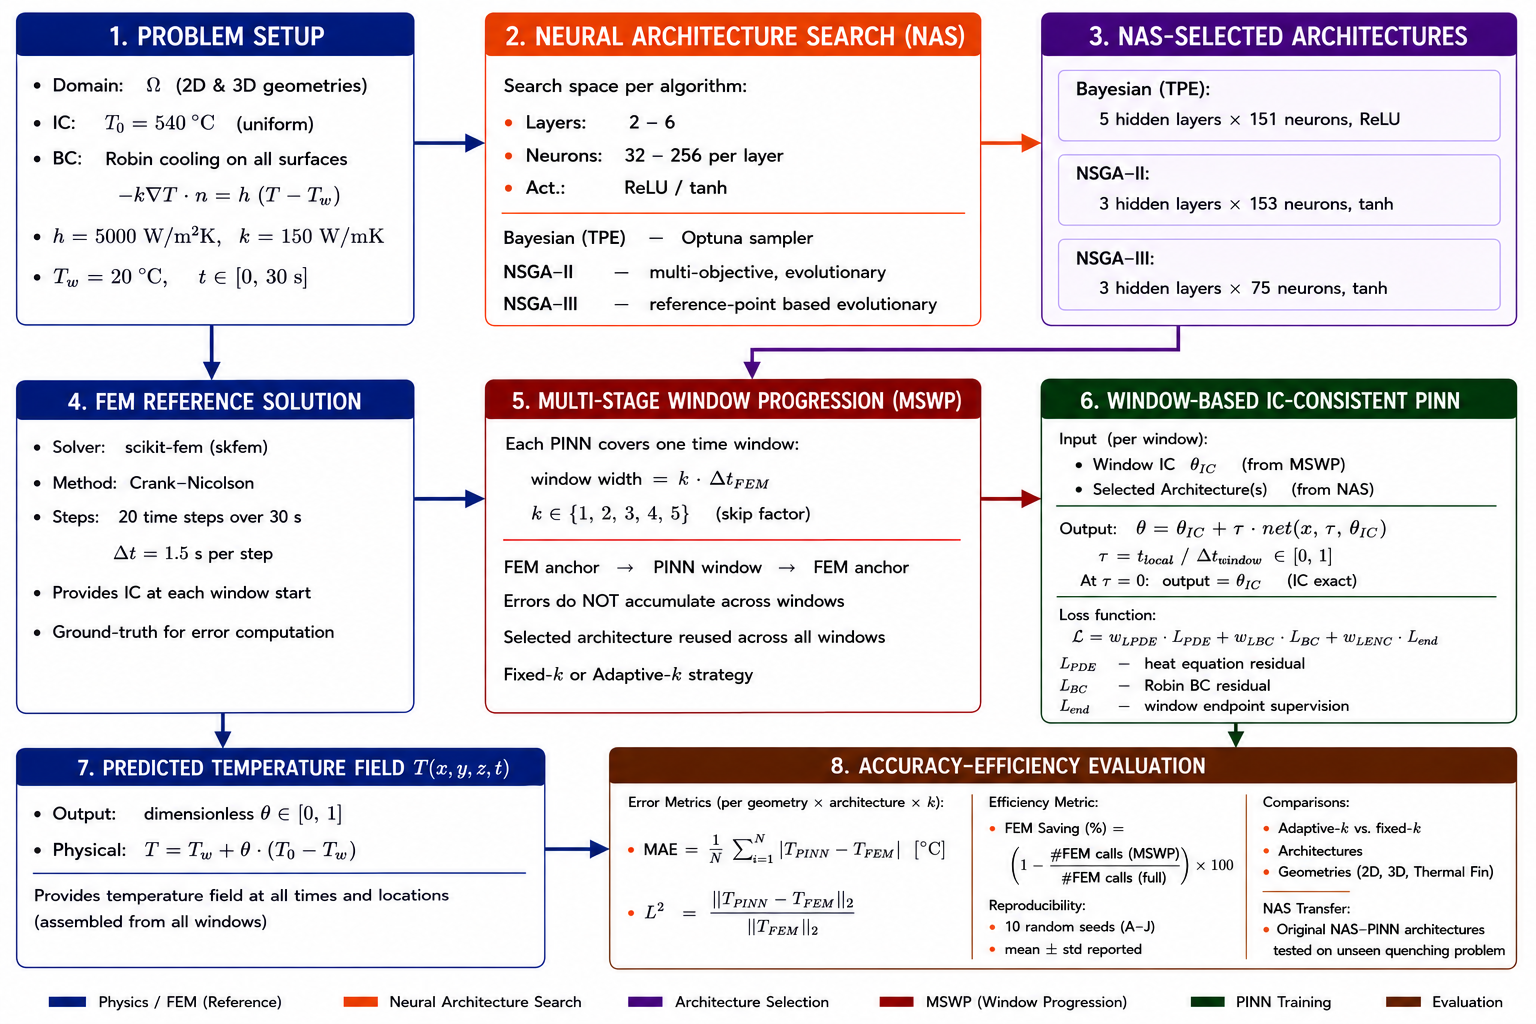
\includegraphics[width=\textwidth]{fig6_naspinn_process.png}
    \end{column}
    \begin{column}{0.41\textwidth}
      \begin{enumerate}\itemsep8pt
        \item \textbf{FEM Reference Solver}\\[2pt]
          {\small Crank--Nicolson FD\\
           Exports every 1.5\,s $\to$ 21 anchors\\
           Called only at anchor points}
        \item \textbf{NAS-PINN}\\[2pt]
          {\small Feed-forward MLP\\
           Architecture from NAS (once)\\
           IC-consistent: $\hat\theta=\theta_\text{ic}+\tau N_\phi$}
        \item \textbf{MSWP Controller}\\[2pt]
          {\small Skip factor $k$: fixed or adaptive\\
           Controls FEM vs.\ PINN budget}
      \end{enumerate}
    \end{column}
  \end{columns}
\end{frame}

\begin{frame}{Methodology: NAS-PINN Architecture}
  \begin{columns}
    \begin{column}{0.50\textwidth}
      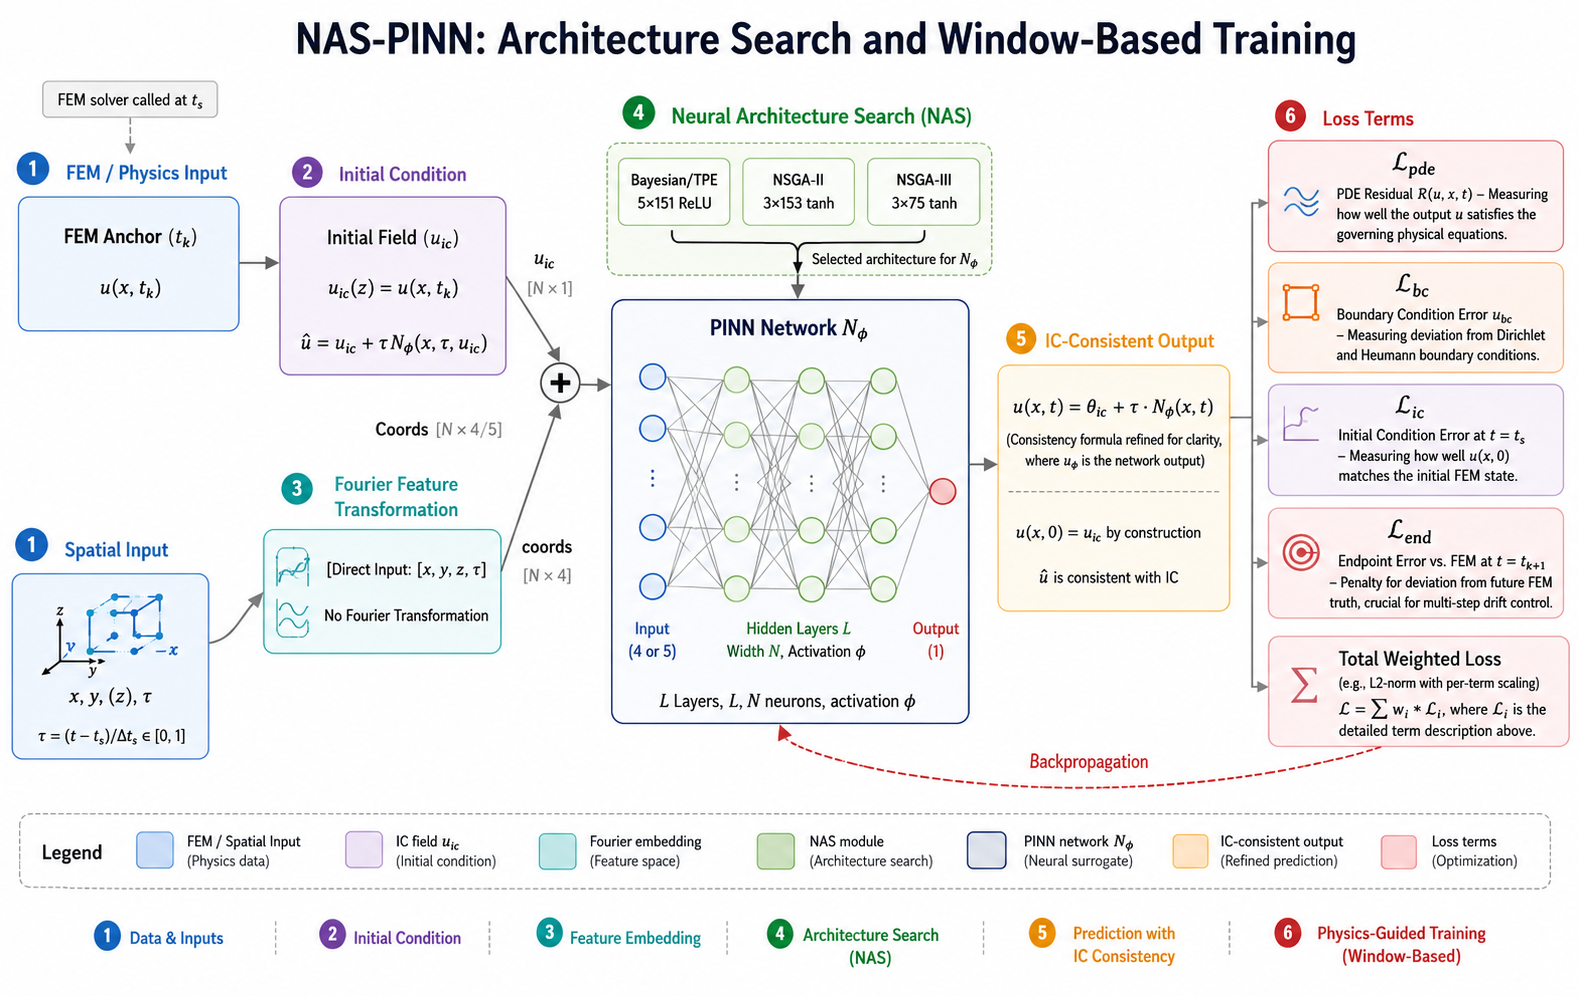
\includegraphics[width=\textwidth]{nas_pinn_framework.png}
    \end{column}
    \begin{column}{0.47\textwidth}
      \textbf{NAS-PINN} (Wang et al., 2023):\\
      standard MLP with NAS-selected architecture.

      \medskip
      \begin{tabular}{ll}
        Layers:     & 2--6\\
        Neurons:    & 32--256 (uniform)\\
        Activation: & ReLU / tanh / SiLU / GELU\\
      \end{tabular}

      \bigskip
      \textbf{Three architectures found:}
      \begin{center}\small
      \begin{tabular}{lcr}
        \toprule
        Strategy & Network & Params\\
        \midrule
        Bayesian/TPE & $5\!\times\!151$ ReLU & 93K\\
        NSGA-II      & $3\!\times\!153$ tanh & 48K\\
        NSGA-III     &  $3\!\times\!75$ tanh & 12K\\
        \bottomrule
      \end{tabular}
      \end{center}

      \medskip
      \alert{NAS run once on rectangle $\to$ deployed on all 10 geometries}
    \end{column}
  \end{columns}
\end{frame}

\begin{frame}{Methodology: MSWP Prediction Loop}
  \begin{columns}
    \begin{column}{0.50\textwidth}
      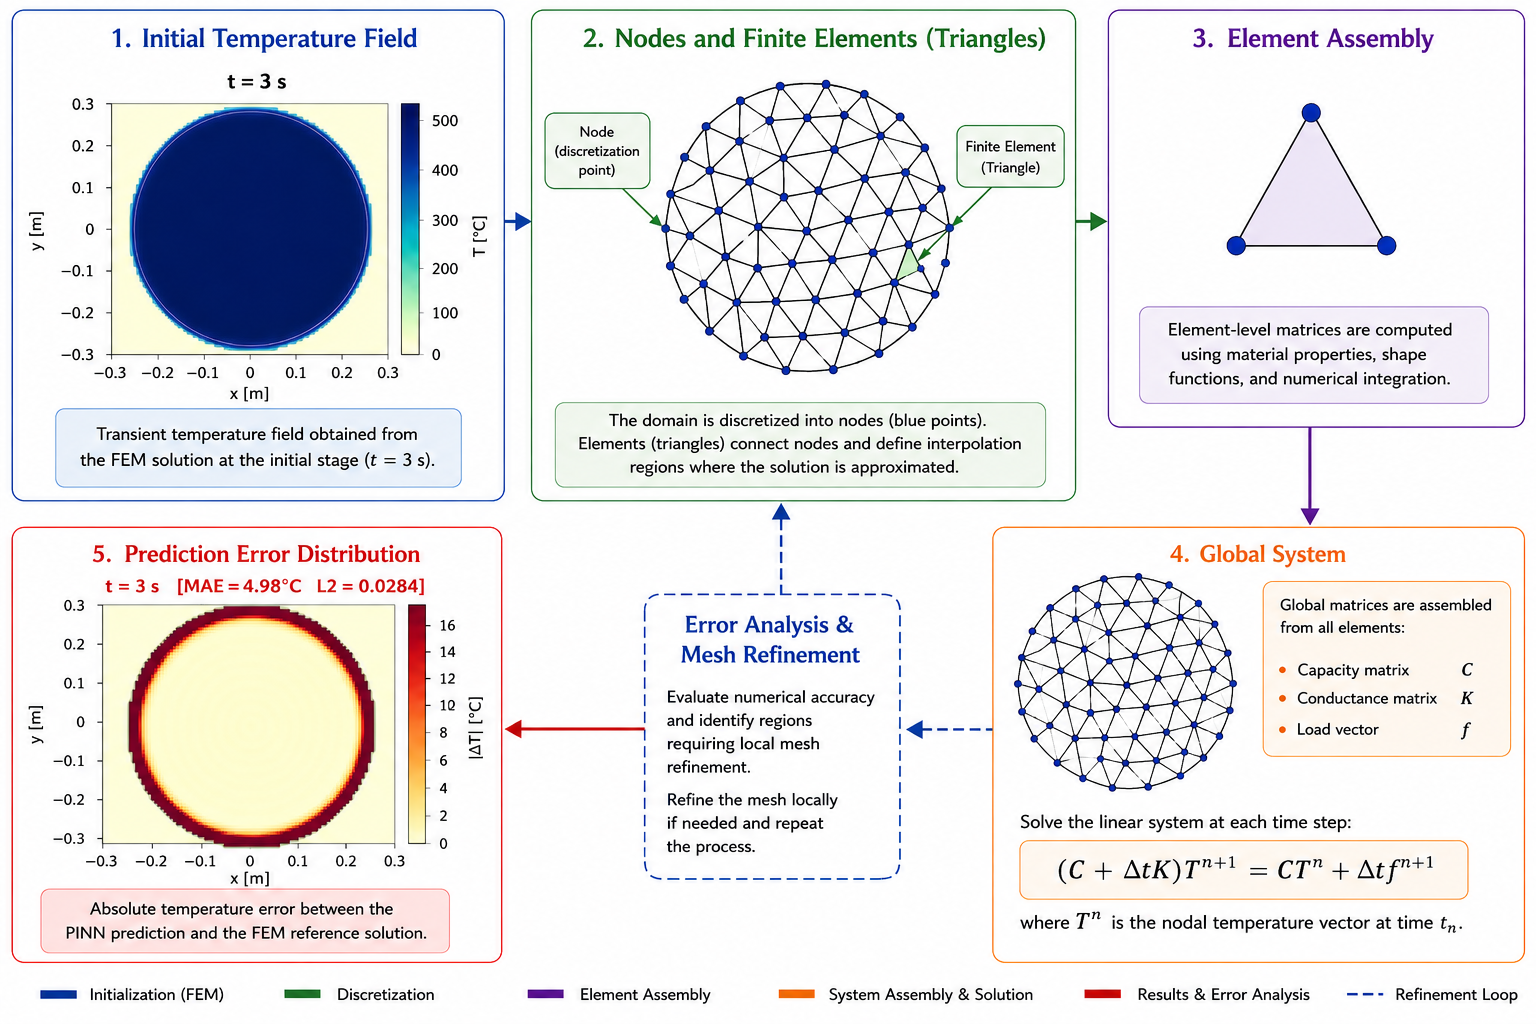
\includegraphics[width=\textwidth]{FEM_Proses.png}
    \end{column}
    \begin{column}{0.47\textwidth}
      \textbf{Algorithm 1 — FEM-anchored fixed $k$:}
      \begin{enumerate}\itemsep3pt\small
        \item $\text{IC} \leftarrow T_\text{FEM}(t_i)$\hfill\textit{anchor}
        \item Train PINN over $[t_i,\;t_i+k\Delta t]$
        \item Predict $\hat{T}(t_{i+1})$
        \item $\varepsilon_i \leftarrow \text{MAE}(\hat{T},\;T_\text{FEM})$
        \item Repeat for all 20/$k$ windows
      \end{enumerate}

      \medskip
      \textbf{Algorithm 3 — Adaptive $k$:}
      \begin{itemize}\small
        \item Promote if $\varepsilon < \tau_\text{up}$ (2 windows) $\to k{+}1$
        \item Demote if $\varepsilon > \tau_\text{down}$ $\to k{-}1$
        \item Phase caps: $\leq$2 early / $\leq$4 mid / $\leq$5 late
      \end{itemize}
    \end{column}
  \end{columns}
\end{frame}

\begin{frame}{Methodology: Benchmark Domains}
  \begin{columns}[c]
    \begin{column}{0.28\textwidth}
      \centering
      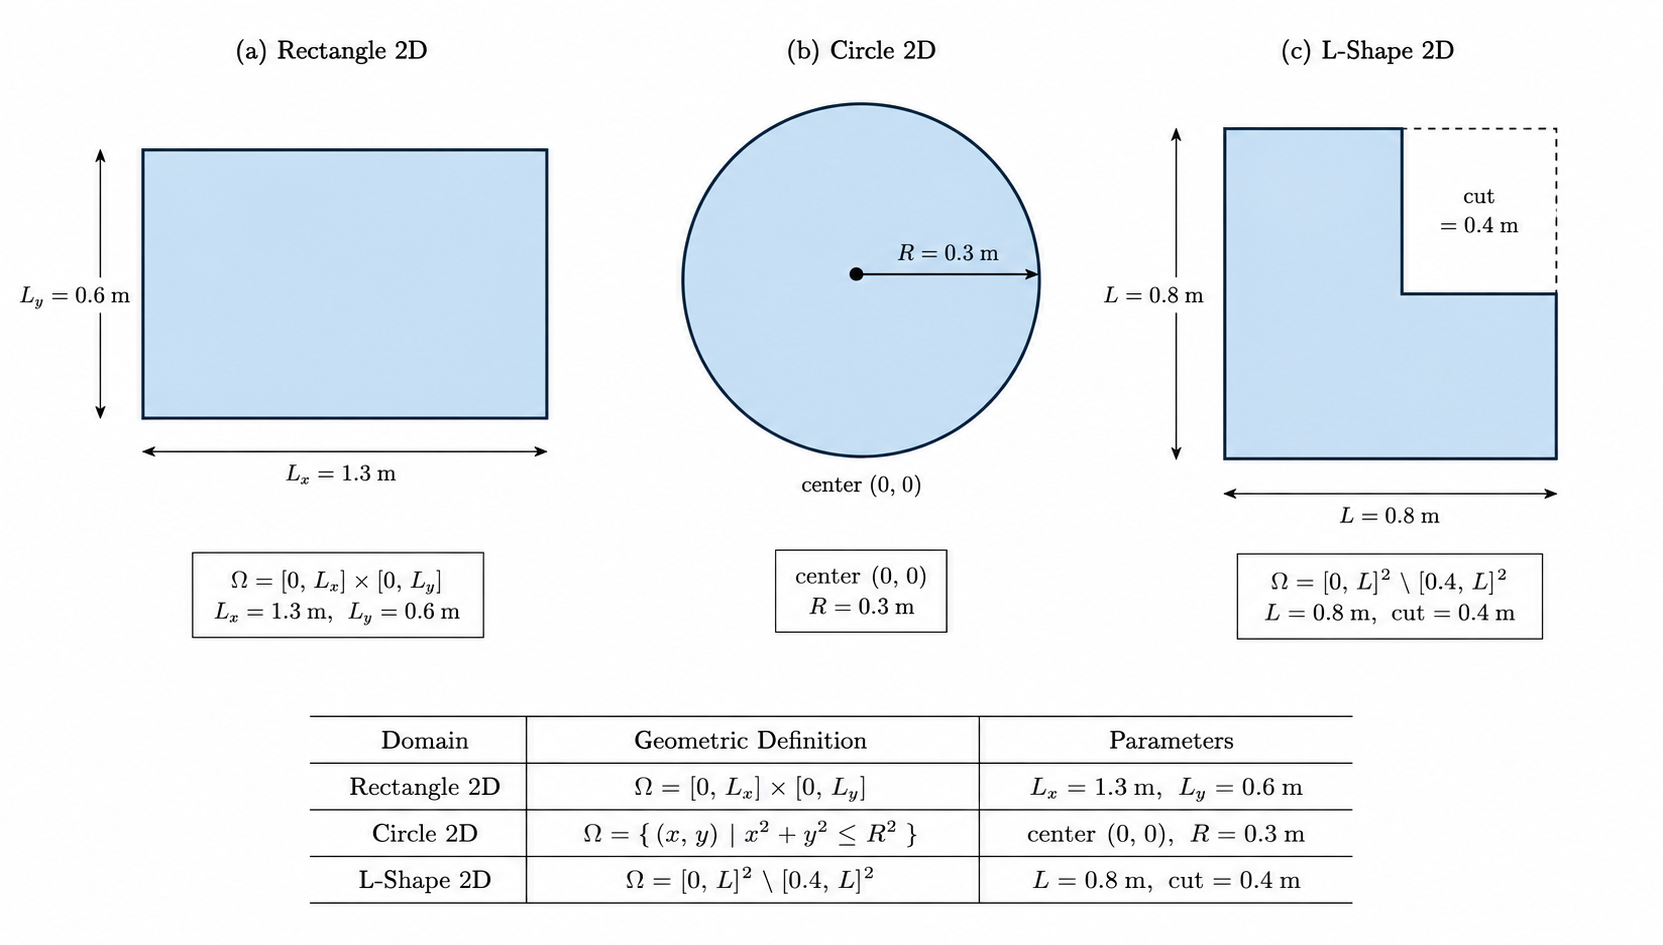
\includegraphics[width=\textwidth]{fig2_thesis_2d.png}\\[4pt]
      {\small\bfseries Canonical 2D}\\
      {\footnotesize\color{textgray}Rectangle $\cdot$ Circle $\cdot$ L-Shape}
    \end{column}
    \begin{column}{0.28\textwidth}
      \centering
      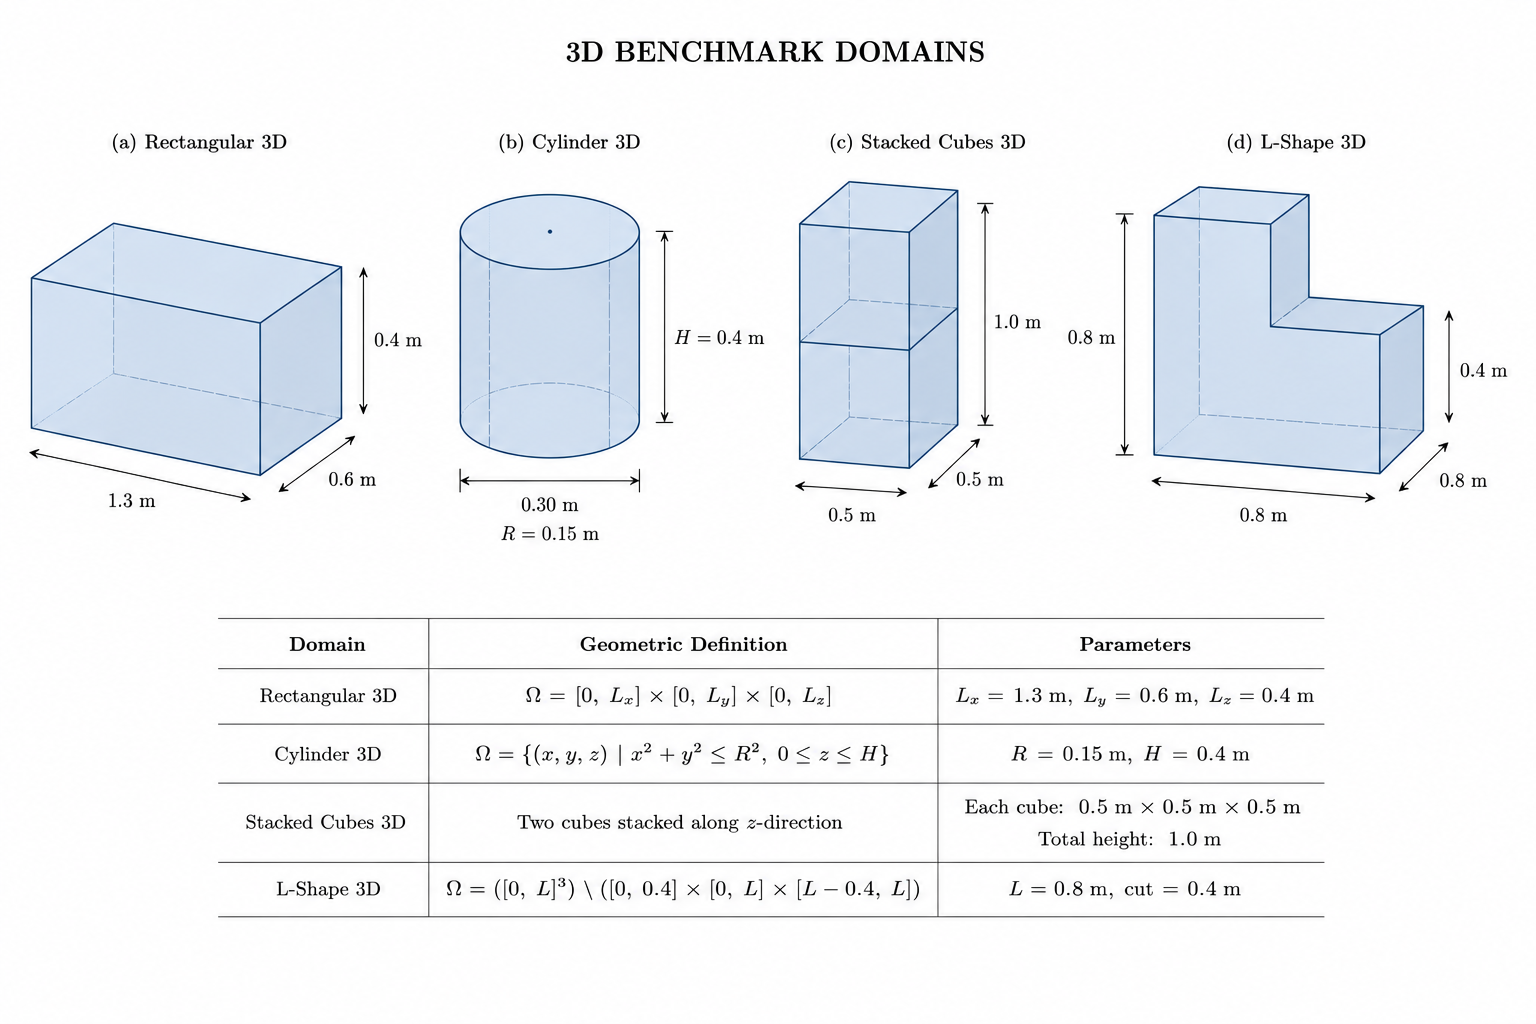
\includegraphics[width=\textwidth]{fig3_thesis_3d.png}\\[4pt]
      {\small\bfseries Canonical 3D}\\
      {\footnotesize\color{textgray}Rectangular $\cdot$ Cylinder\\Stacked $\cdot$ L-Shape Prism}
    \end{column}
    \begin{column}{0.28\textwidth}
      \centering
      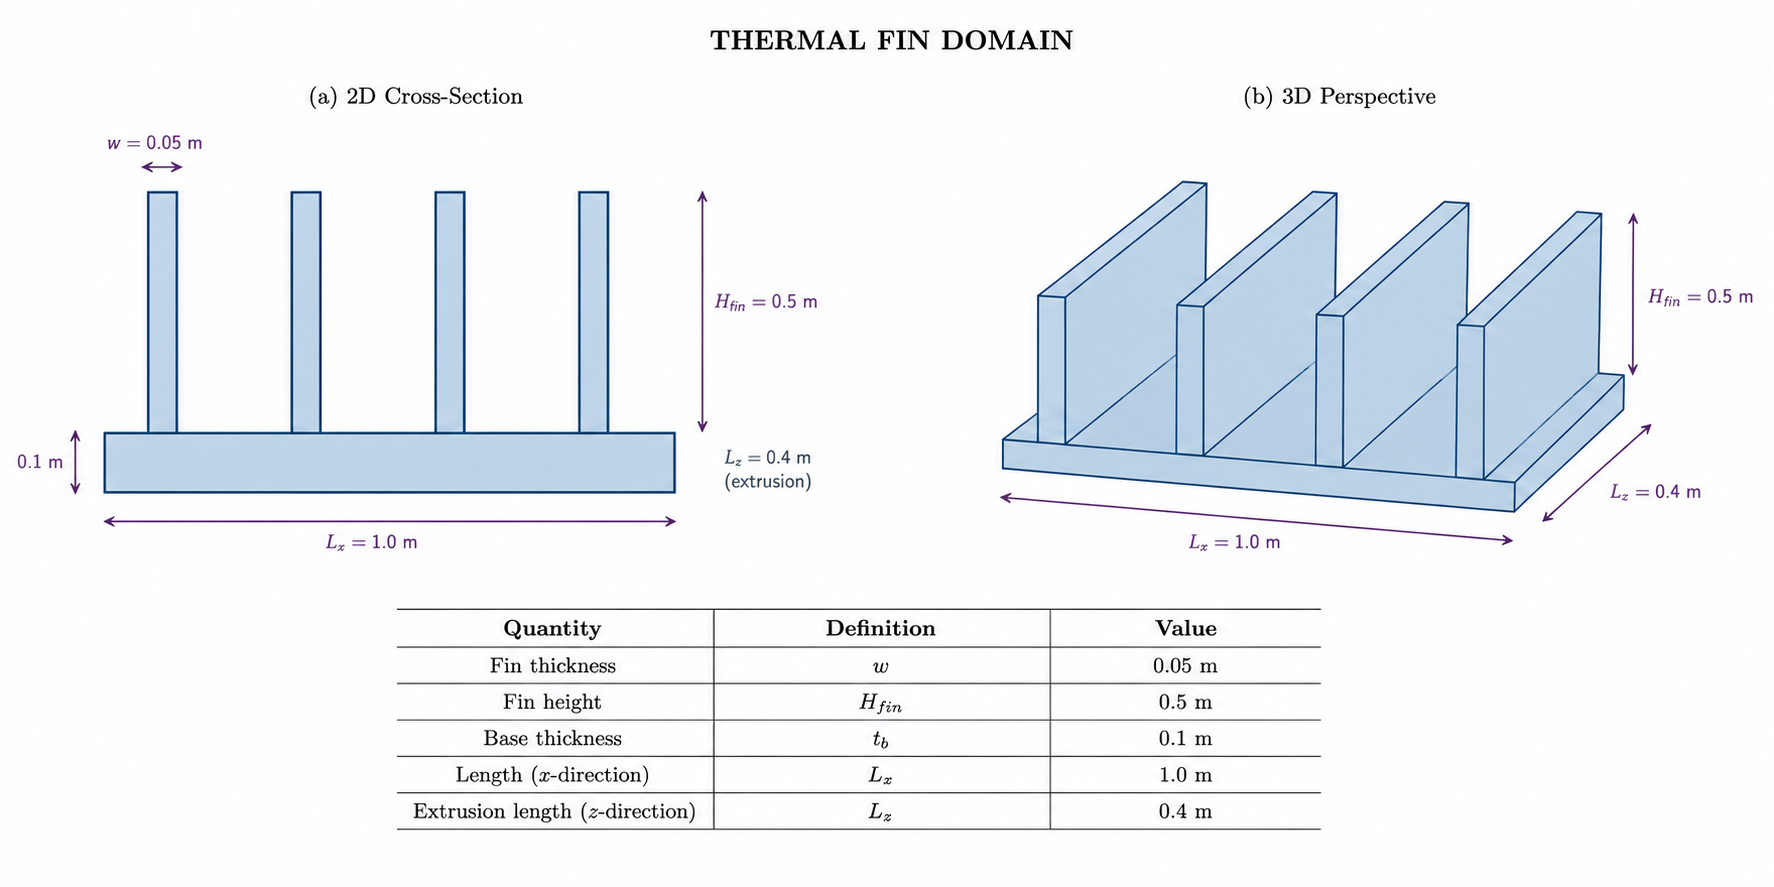
\includegraphics[width=\textwidth]{fig4_thermalfin.png}\\[4pt]
      {\small\bfseries Thermal Fin}\\
      {\footnotesize\color{textgray}RBniCS benchmark\\extended to 3D transient}
    \end{column}
  \end{columns}
  \vspace{6pt}
  \textcolor{ruled}{\rule{\textwidth}{0.4pt}}
  \vspace{2pt}

  {\small
  $T_0=540$\,\textdegree C,\; $T_w=20$\,\textdegree C,\; 30-second quench\quad|\quad
  \textbf{10 seeds} per (domain, architecture, $k$)\quad|\quad
  Adaptive-$k$ adds Square and Flower}
\end{frame}

% ============================================================
\sectionslide{03\quad Results}{2D $\cdot$ Adaptive-$k$ $\cdot$ 3D $\cdot$ Thermal Fin $\cdot$ PINN-only}
% ============================================================

\begin{frame}{Results: 2D Canonical — Fixed-$k$ Sweep}
  \begin{columns}
    \begin{column}{0.50\textwidth}
      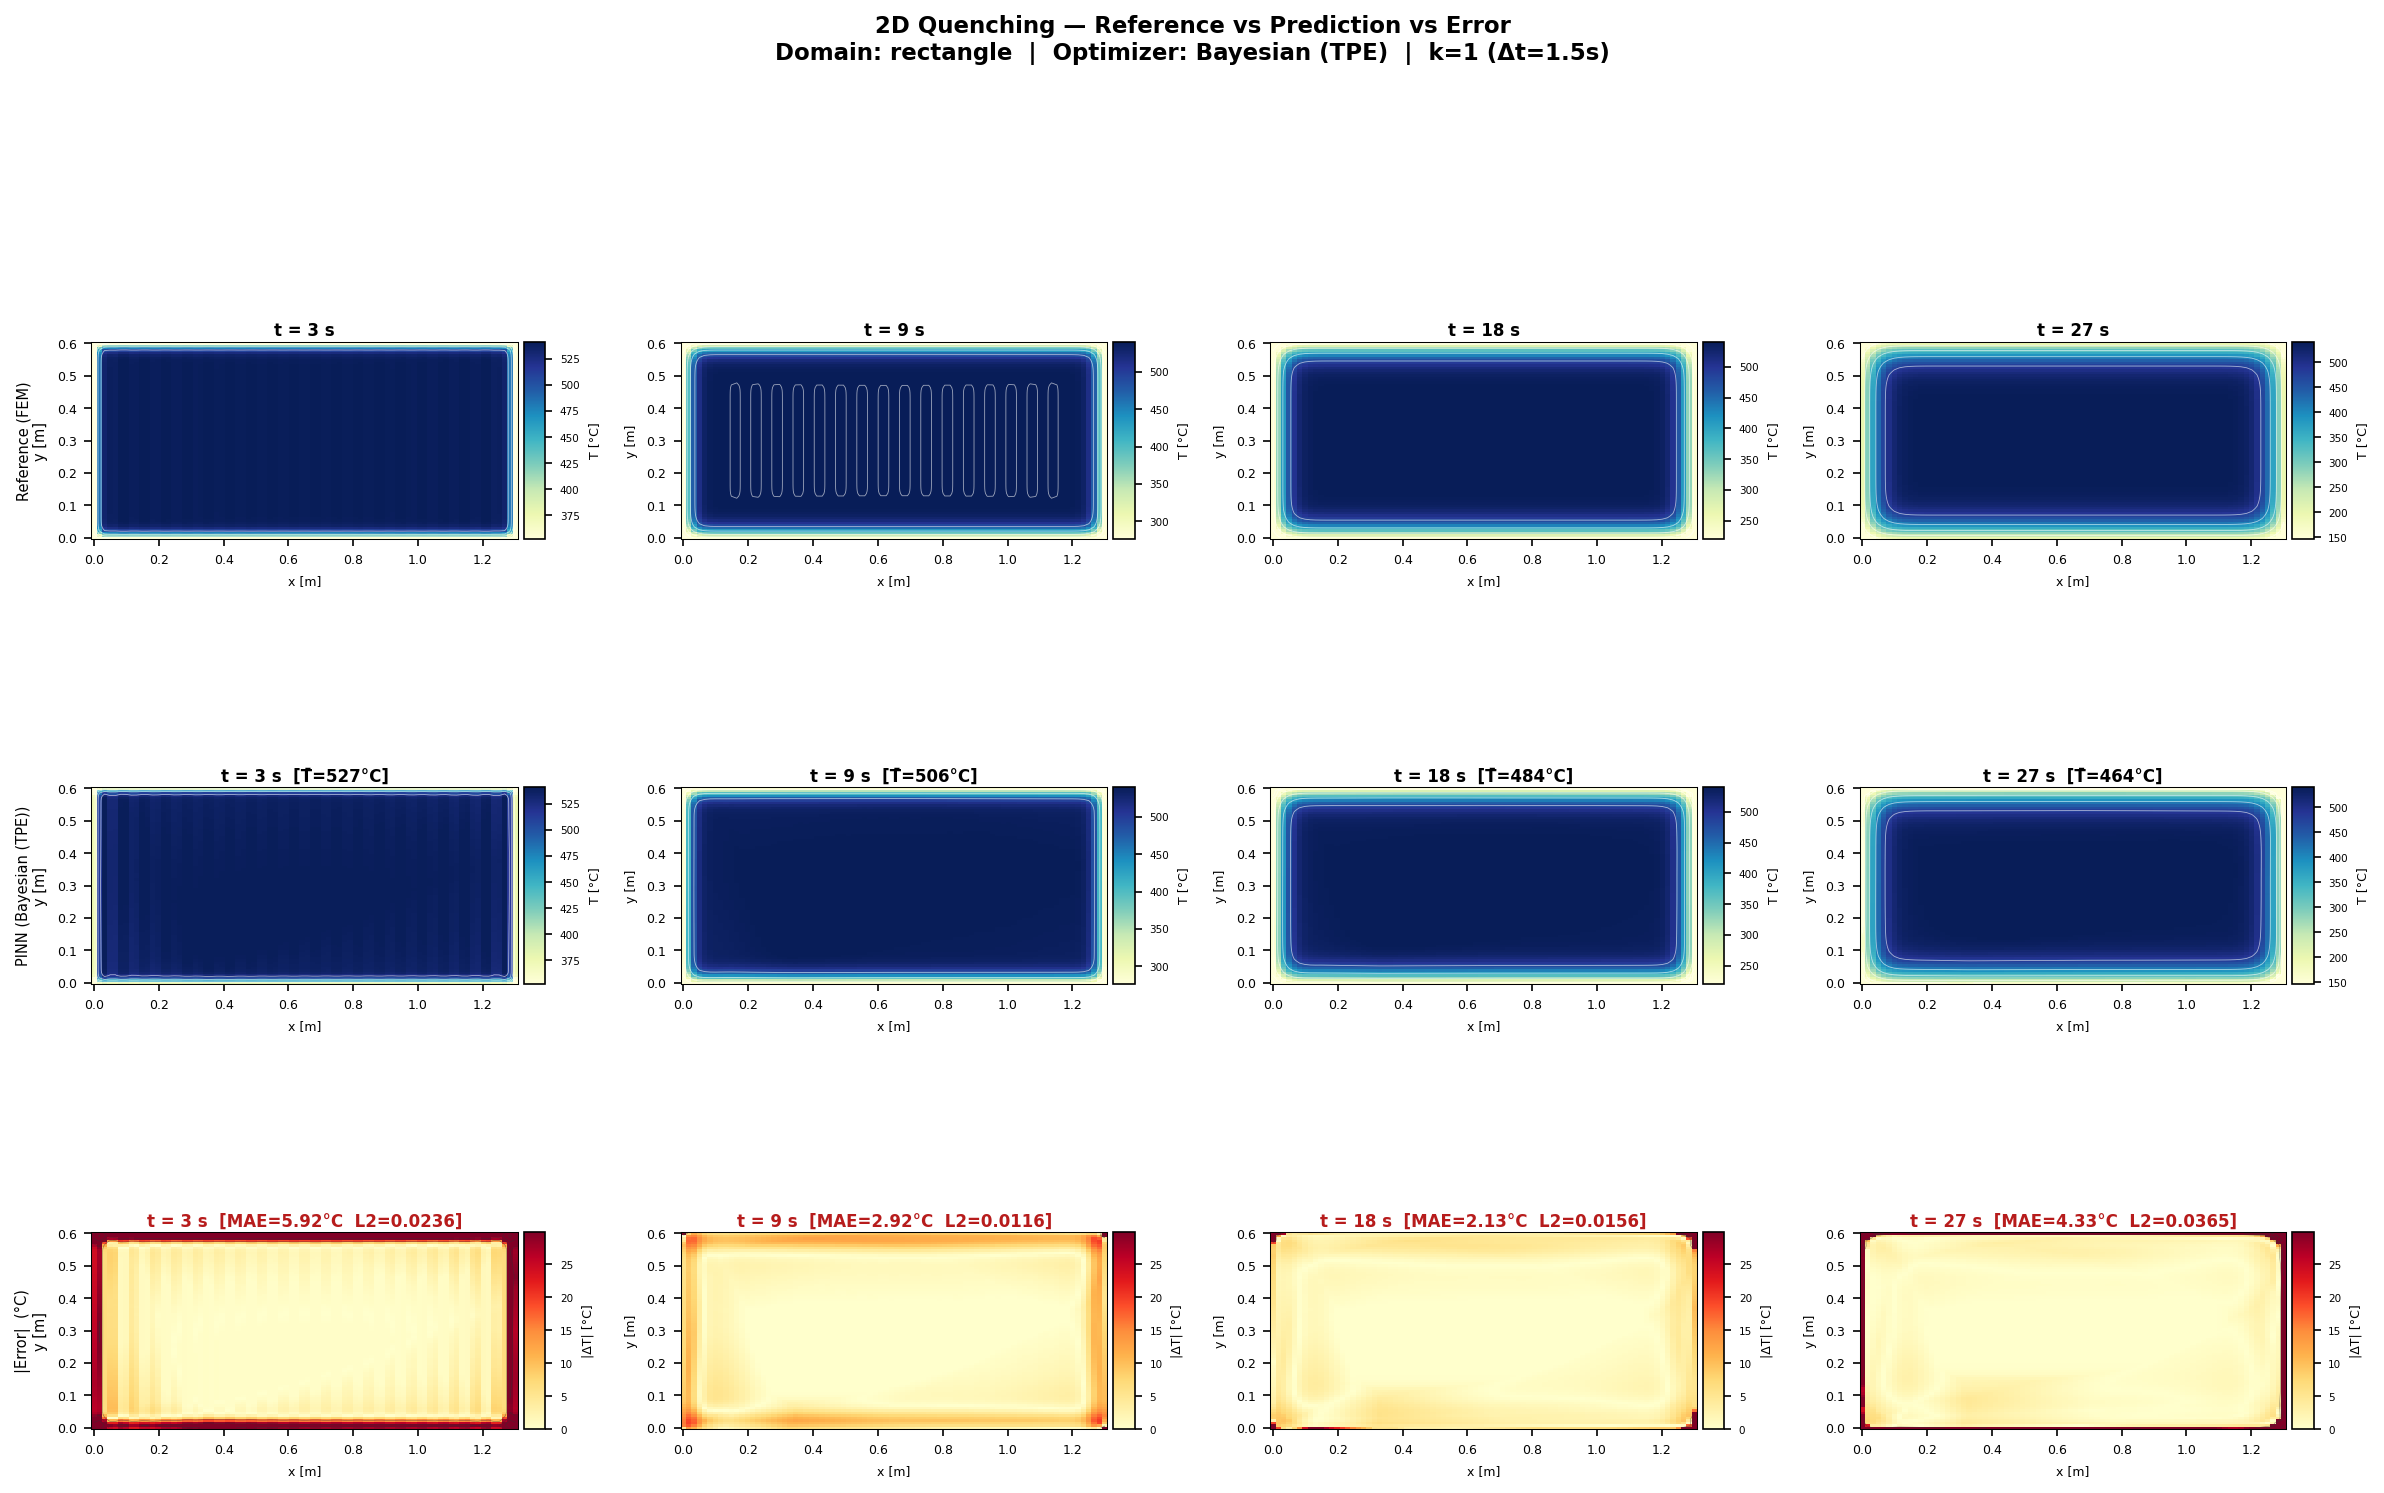
\includegraphics[width=\textwidth]{2d_bestk_bayesian_rectangle.png}
    \end{column}
    \begin{column}{0.47\textwidth}
      \textbf{Bayesian/TPE} ($5\!\times\!151$, ReLU):
      \begin{itemize}
        \item $\leq 5$\,\textdegree C through $k=3$ on \emph{all} 3 domains\\
              $\Rightarrow$ \textbf{65\% FEM saving} \checkmark
        \item Rectangle / L-Shape $k=5$: $<6$\,\textdegree C \checkmark
        \item Circle $k=5$: 10\,\textdegree C \quad(curved normals)
      \end{itemize}

      \medskip
      \textbf{NSGA-II / NSGA-III:}
      \begin{itemize}
        \item Reliable through $k=3$ (65\% saving)
        \item L-Shape $k=5$: up to 14.4\,\textdegree C \quad$\times$
        \item Compact tanh saturates on long windows
      \end{itemize}

      \medskip
      \begin{alertblock}{Interpolation baseline}
        \small Lower $L_2$ on smooth domains —
        PINN advantage appears at complex geometry
        (L-Shape, Flower, Stacked Cubes).
      \end{alertblock}
    \end{column}
  \end{columns}
\end{frame}

\begin{frame}{Results: 2D Adaptive-$k$}
  \begin{columns}
    \begin{column}{0.50\textwidth}
      
\includegraphics[width=\textwidth]{fem_pinn_adaptive_k_lshape.png}
    \end{column}
    \begin{column}{0.47\textwidth}
      \textbf{4 domains, all 4 architectures:}
      \begin{itemize}
        \item \textbf{83--85\% FEM saving}, MAE $<2.5$\,\textdegree C \checkmark
        \item All architectures follow the \emph{same} $k$-schedule
      \end{itemize}

      \medskip
      \begin{block}{Key insight}
        \small The controller responds to the physics of cooling,
        not to architecture-specific artefacts.
      \end{block}

      \medskip
      \textbf{L-Shape exception:}
      \begin{itemize}
        \item Bayesian/TPE: 1.36\,\textdegree C \checkmark
        \item NSGA-II/III: 2.34--2.44\,\textdegree C
        \item Reentrant corner needs large ReLU capacity
      \end{itemize}
    \end{column}
  \end{columns}
\end{frame}

\begin{frame}{Results: 3D Canonical Domains}
  \begin{columns}
    \begin{column}{0.50\textwidth}
      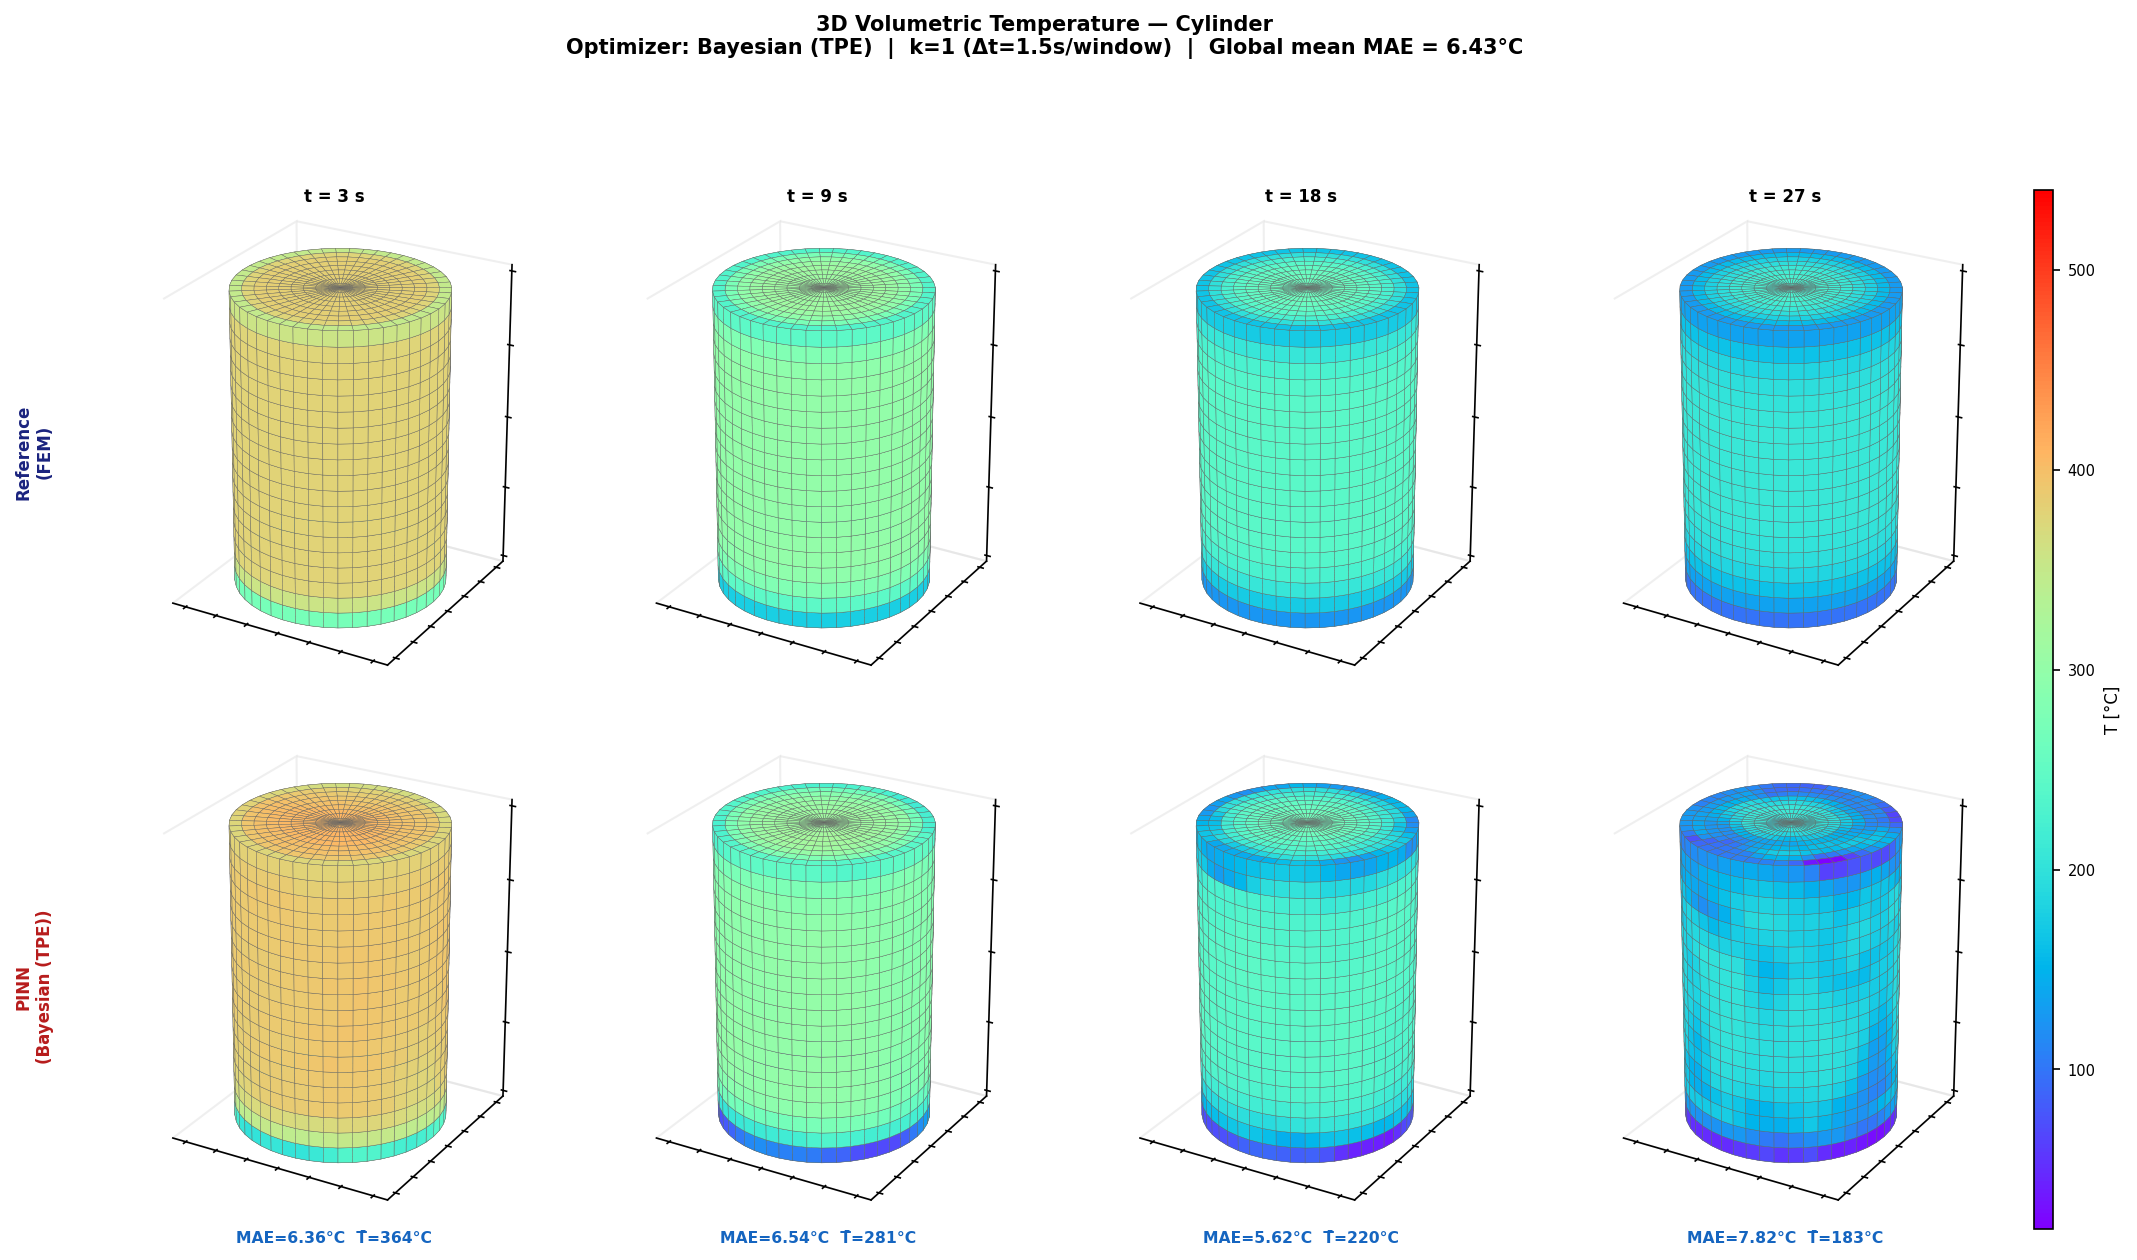
\includegraphics[width=\textwidth]{3d_bestk_bayesian_cylinder.png}
    \end{column}
    \begin{column}{0.47\textwidth}
      \textbf{Bayesian/TPE:} $k=5$ on all 4 domains, all $<15$\,\textdegree C\\
      $\Rightarrow$ \textbf{80\% FEM saving} \checkmark

      \medskip
      \textbf{NSGA-II failure on Cylinder:}
      \begin{itemize}
        \item $\sigma=12.3$\,\textdegree C at $k=5$ (high variance)
        \item Curved normals + tanh saturation + compact loss landscape
      \end{itemize}

      \medskip
      \textbf{Interesting finding on 3D L-Shape:}
      \begin{itemize}
        \item NSGA-III beats Bayesian at $k=1$
        \item Localised edge gradient matches tanh bias
        \item Advantage disappears at $k=5$
      \end{itemize}

      \medskip
      \begin{alertblock}{$k_5/k_1$ error ratio}
        \small 3D Bayesian: 1.2--2.5 \quad (rich structure helps)\\
        2D compact: 4.8--7.6 \quad (long windows cause drift)
      \end{alertblock}
    \end{column}
  \end{columns}
\end{frame}

\begin{frame}{Results: Thermal Fin Benchmark}
  \begin{columns}
    \begin{column}{0.50\textwidth}
      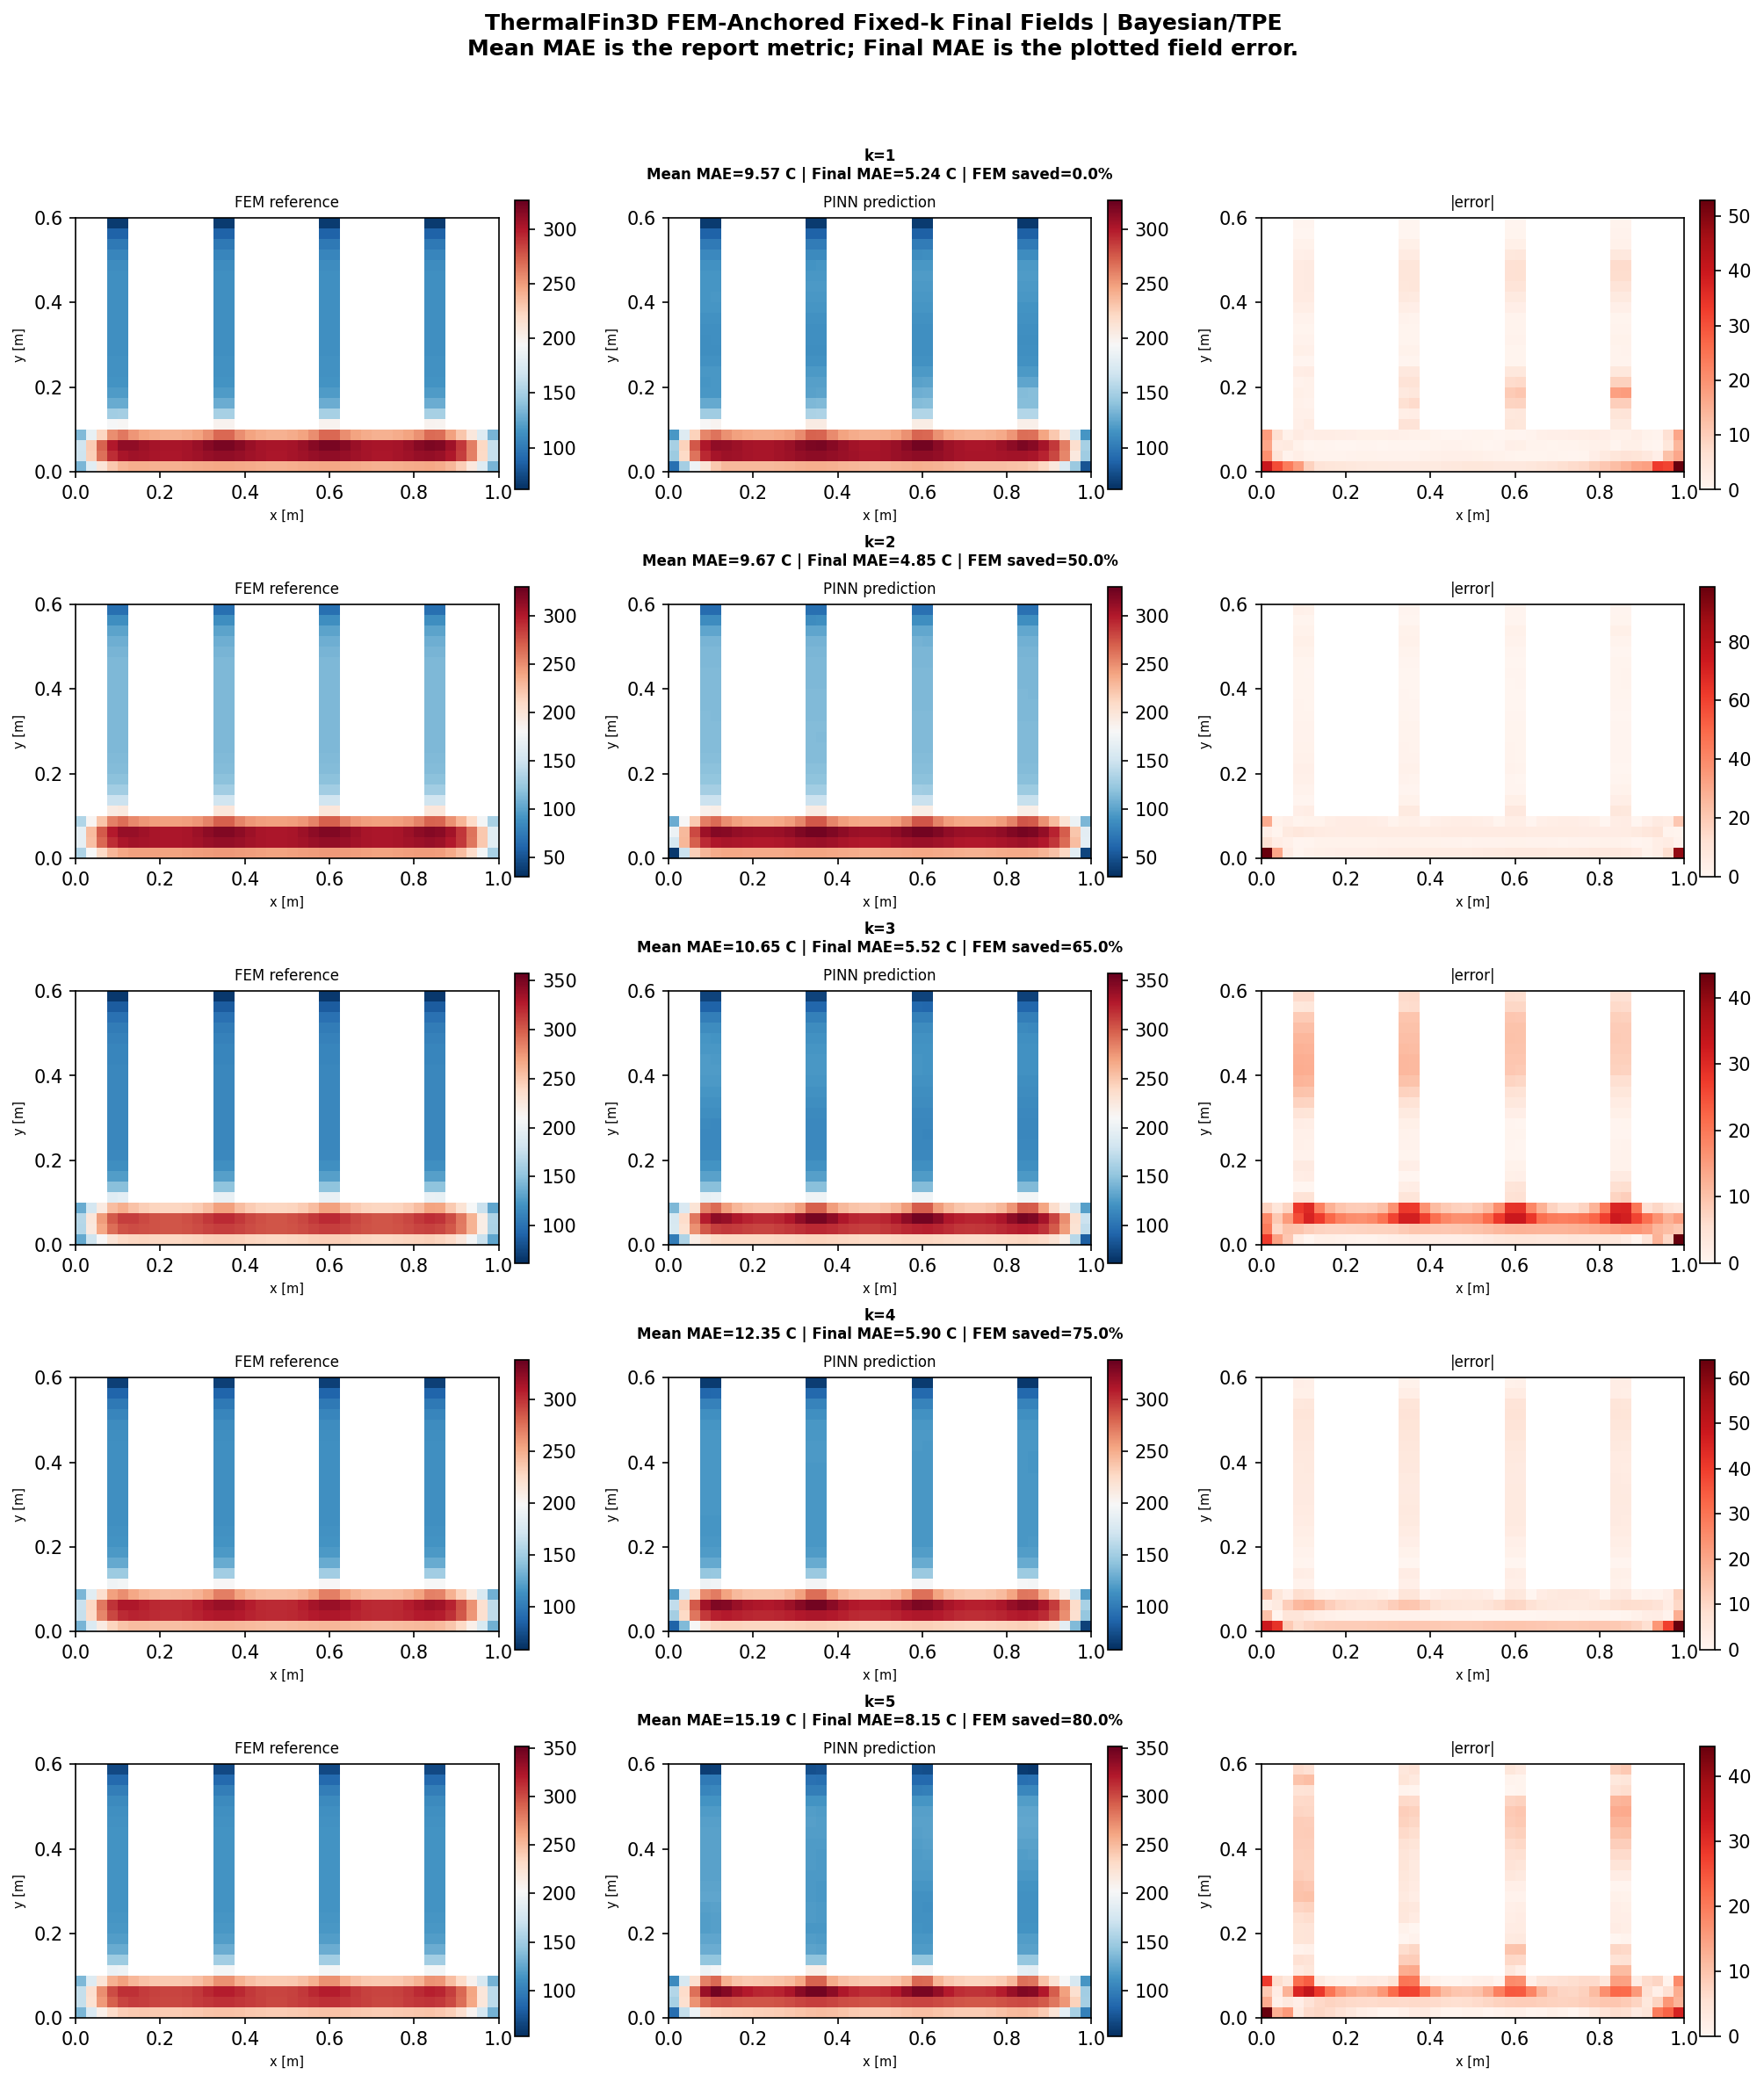
\includegraphics[width=\textwidth]{thermal_fin_bayesian_fixed_k_clean_heatmaps.png}
    \end{column}
    \begin{column}{0.47\textwidth}
      {\small Hardest geometry: 3D fin, 22 surfaces, fin-tip gradient,
      threshold 15\,\textdegree C}

      \medskip
      \textbf{Fixed-$k$ results:}
      \begin{itemize}
        \item Bayesian + Fourier: $k=5\to12.55$\,\textdegree C \checkmark \,(80\%)
        \item NSGA-II/III: $k=4\to14.1$--$14.4$\,\textdegree C \checkmark \,(75\%)
        \item NSGA at $k=5$: 15.56/15.74\,\textdegree C \quad$\times$
      \end{itemize}

      \medskip
      \textbf{Fourier embedding:}
      \begin{itemize}
        \item Reduces Bayesian error by 1.8--4.4\,\textdegree C
        \item Detrimental for compact 3-layer NSGA networks
      \end{itemize}

      \medskip
      \begin{block}{First window hardest}
        \small Fin-tip cools instantly at onset, interior still at 540\,\textdegree C.
        Mean-window MAE averages steep early + easier late phase.
      \end{block}
    \end{column}
  \end{columns}
\end{frame}

\begin{frame}{Results: PINN-Only Mode}
  \begin{columns}
    \begin{column}{0.50\textwidth}
      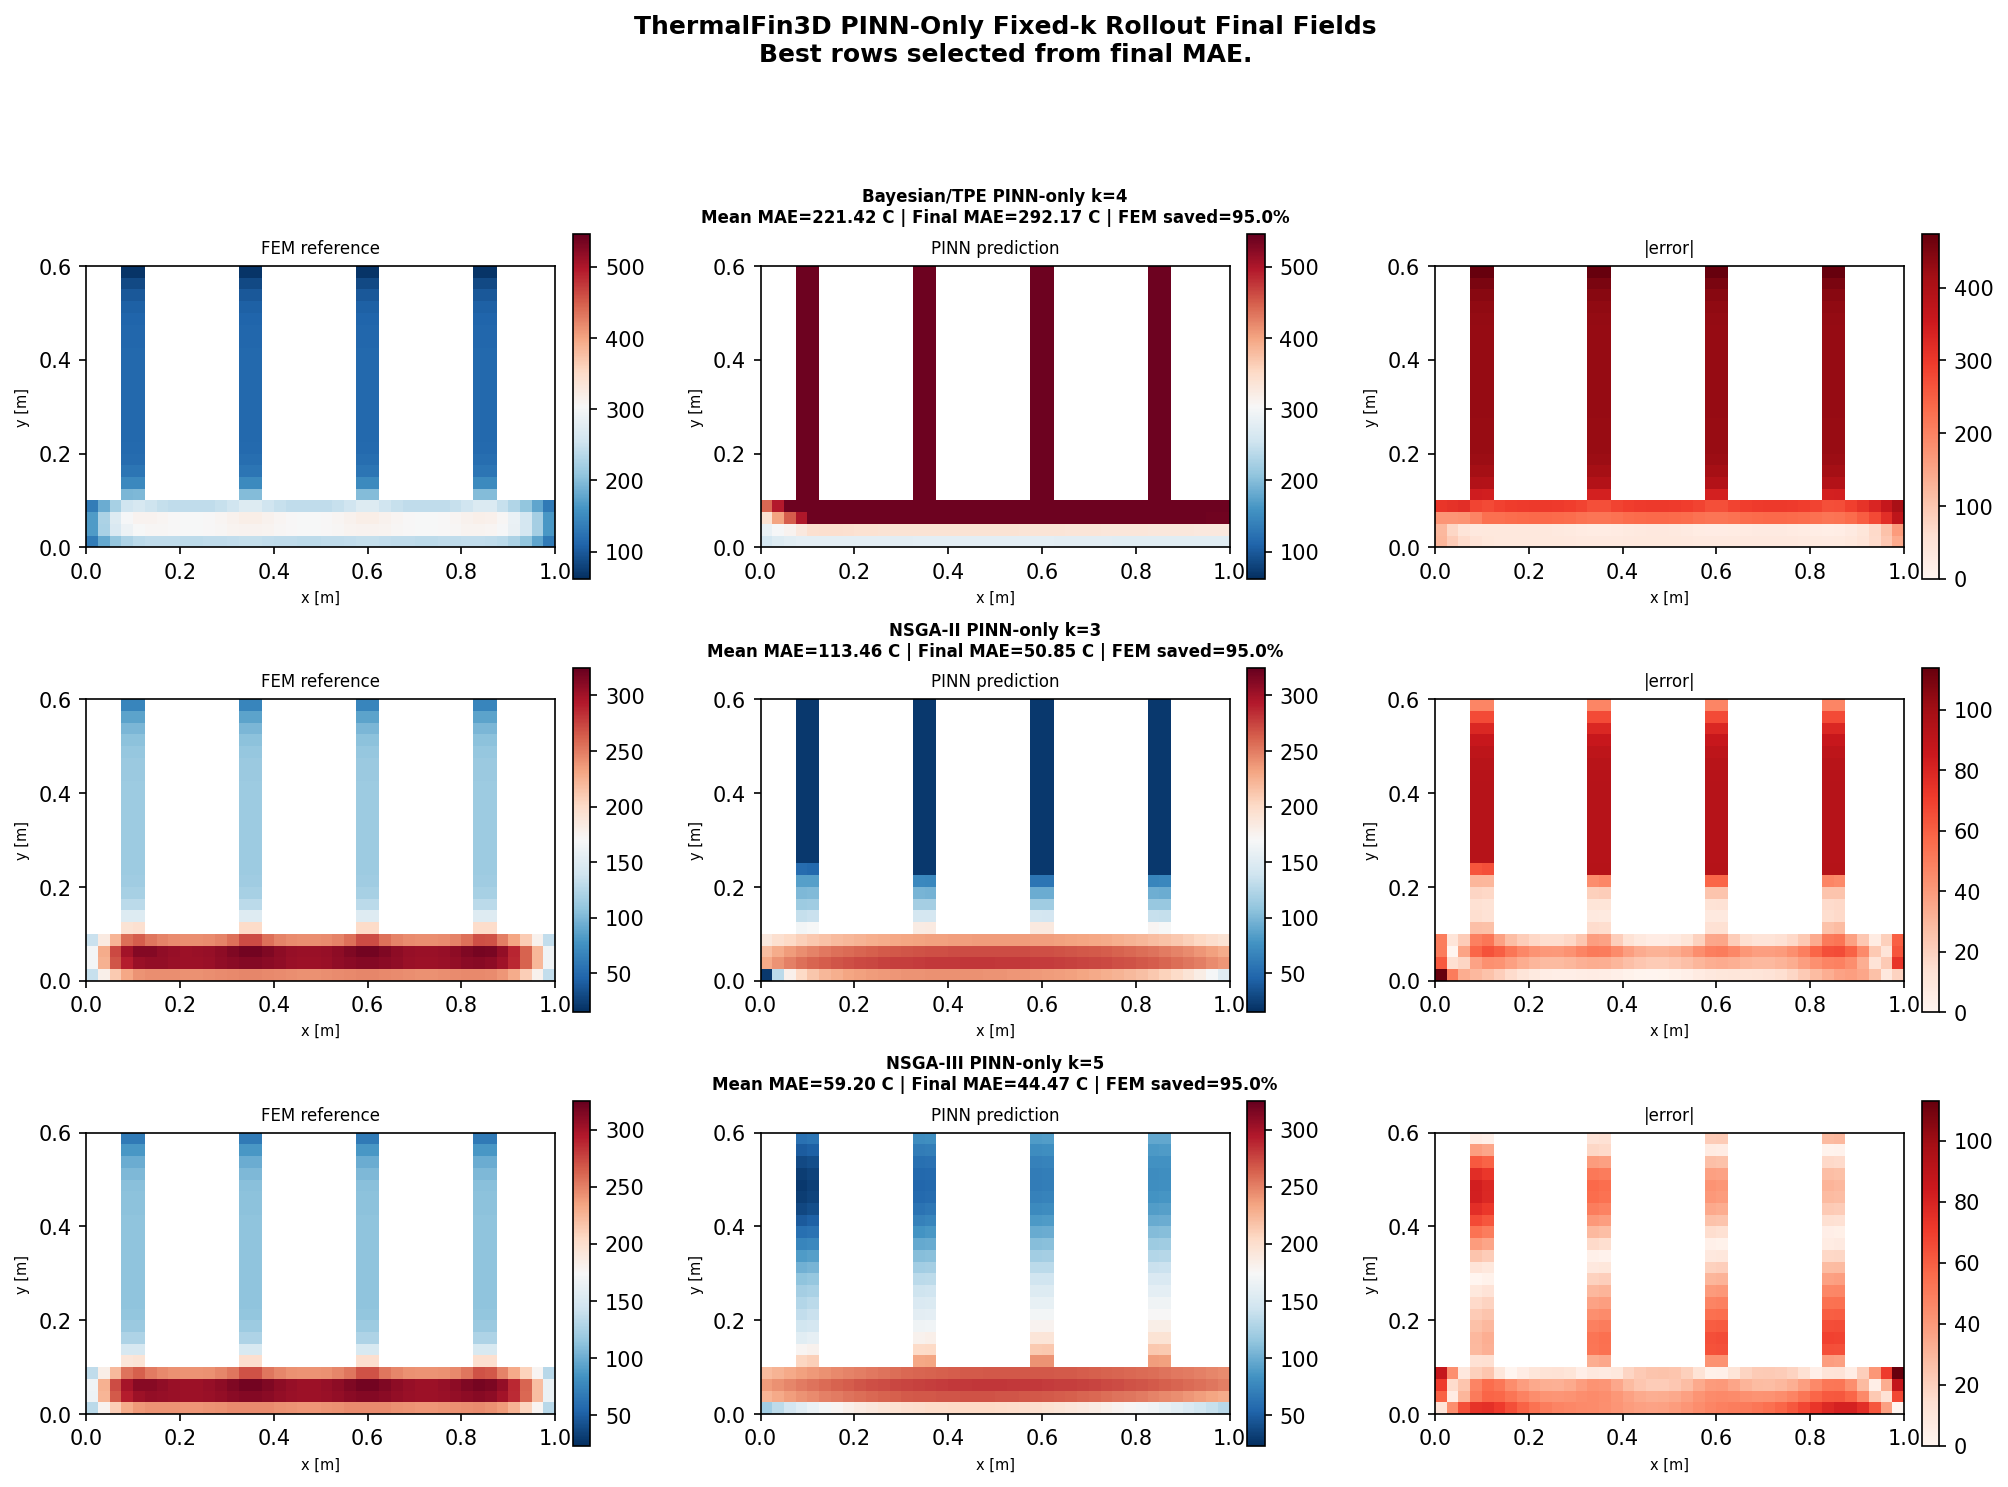
\includegraphics[width=\textwidth]{thermal_fin_pinn_only_best_clean_heatmaps.png}
    \end{column}
    \begin{column}{0.47\textwidth}
      FEM corrections removed $\to$ PINN-only rollout:

      \medskip
      \begin{center}\small
      \begin{tabular}{lccc}
        \toprule
        & Anchored & PINN-only & Factor\\
        \midrule
        2D Square & 1.6\,\textdegree C & 29.6\,\textdegree C & $\times$18\\
        TF NSGA   & 14.1\,\textdegree C & 59.2\,\textdegree C & $\times$4\\
        TF Bayes  & 12.6\,\textdegree C & $>$200\,\textdegree C & diverges\\
        \bottomrule
      \end{tabular}
      \end{center}

      \medskip
      Large Bayesian network fails \emph{fastest} —
      more expressive $\Rightarrow$ drift accumulates faster without reset.

      \medskip
      \begin{block}{\textbf{Conclusion}}
        FEM anchoring is a \textbf{structural requirement}.\\
        This is a FEM-\emph{reduction} strategy,\\
        not FEM-\emph{replacement}.
      \end{block}
    \end{column}
  \end{columns}
\end{frame}

% ============================================================
\sectionslide{04\quad Discussion}{Cross-domain analysis $\cdot$ Practical guidance}
% ============================================================

\begin{frame}{Discussion: Cross-Domain Analysis}
  \begin{columns}
    \begin{column}{0.50\textwidth}
      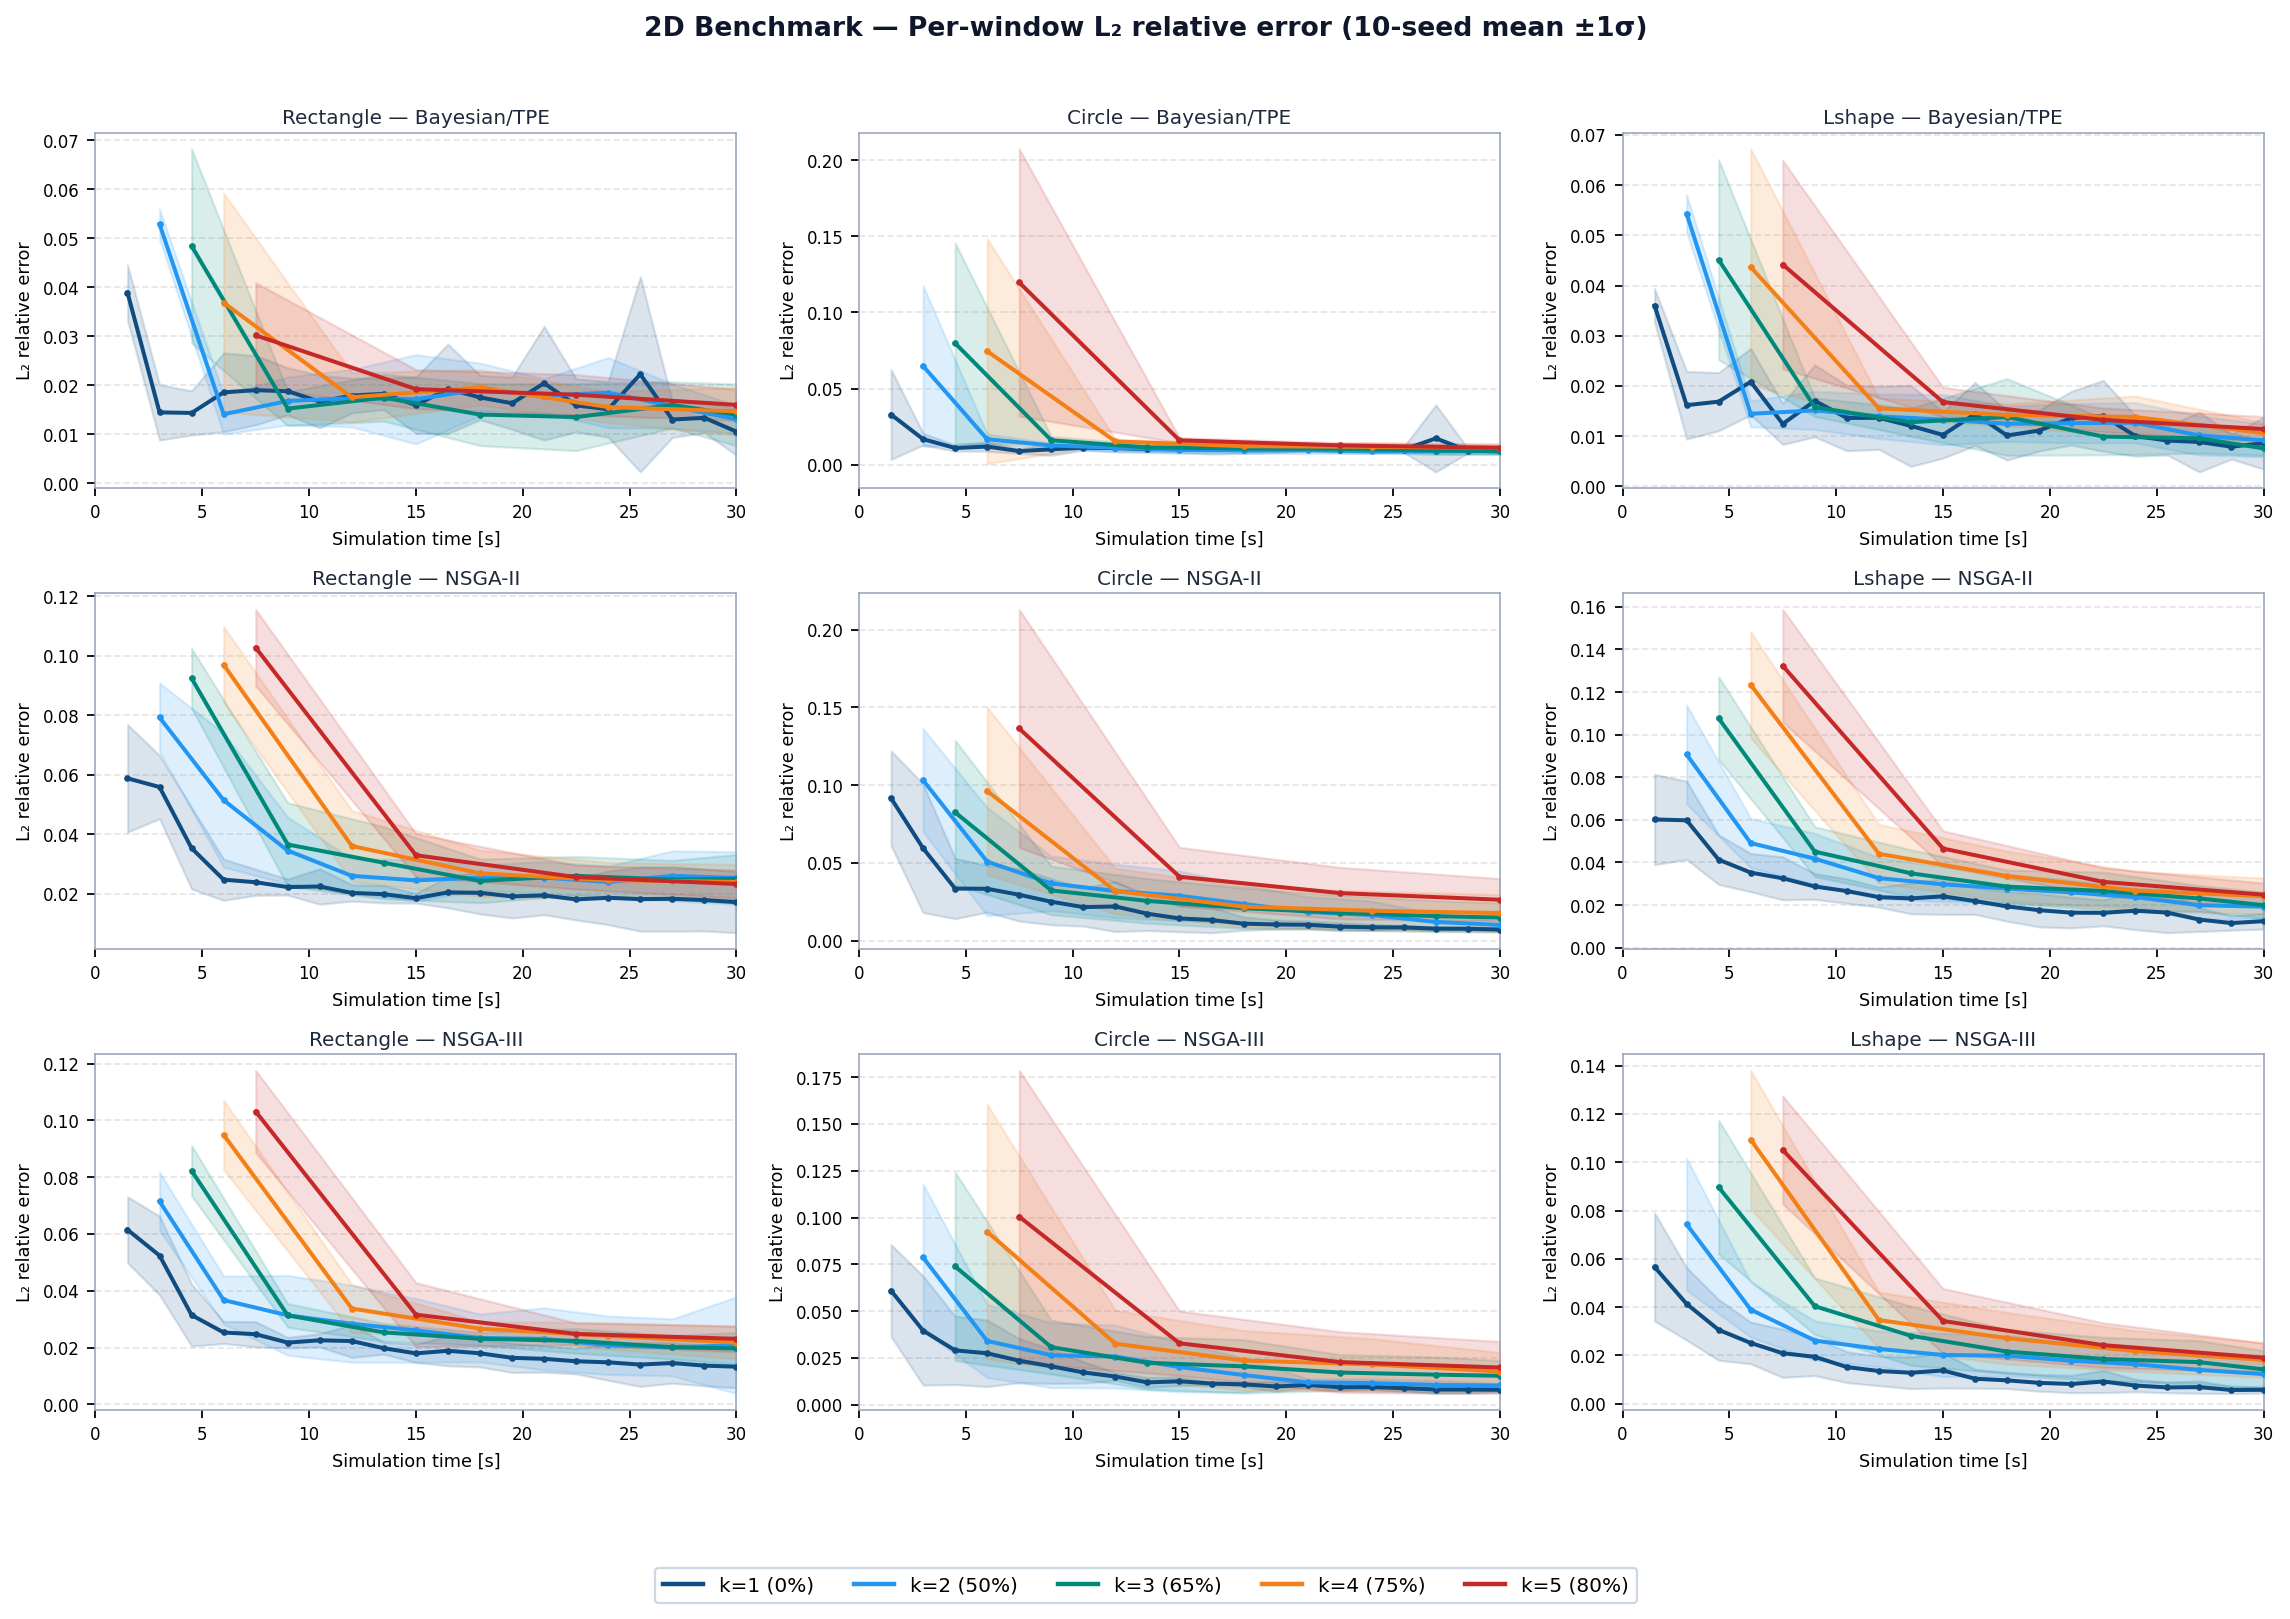
\includegraphics[width=\textwidth]{l2_all_k_2d.png}
    \end{column}
    \begin{column}{0.47\textwidth}
      \textbf{Bayesian/TPE dominates:}
      \begin{itemize}
        \item 7/8 canonical domains at $k=5$ within threshold
        \item Transfers from rectangle to all 10 geometries
      \end{itemize}

      \medskip
      \textbf{Practical guidance:}

      \smallskip
      \begin{tabular}{lp{4.5cm}}
        \textit{Simple 2D:}    & adaptive-$k$, any arch.\\
                               & 83--85\% saving, MAE $<2.5$\,\textdegree C\\[4pt]
        \textit{Complex 3D:}   & fixed $k=4$--$5$, Bayesian/TPE\\
                               & 75--80\% saving, MAE $<15$\,\textdegree C\\
      \end{tabular}

      \medskip
      \begin{alertblock}{Industrial mesh estimate}
        \small $k=4$: 40\,min $\to$ 10\,min per simulation\\
        100 design runs: 67\,h $\to$ \textbf{17\,h} saved
      \end{alertblock}
    \end{column}
  \end{columns}
\end{frame}

% ============================================================
\sectionslide{05\quad Conclusion}{Summary $\cdot$ Contributions $\cdot$ Future steps}
% ============================================================

\begin{frame}{Conclusion: Summary of Findings}
  \begin{columns}[t]
    \begin{column}{0.48\textwidth}
      \begin{block}{Main Results}
        \begin{itemize}
          \item \textbf{65--85\%} FEM saving within 15\,\textdegree C
          \item Bayesian/TPE: $k=5$ on 7/8 domains
          \item Adaptive-$k$: 83--85\% on all 2D
        \end{itemize}
      \end{block}
      \vspace{6pt}
      \begin{block}{Architecture}
        \begin{itemize}
          \item Bayesian/TPE most robust across all geometries
          \item Geometry-specific NAS adds value on irregular shapes
        \end{itemize}
      \end{block}
    \end{column}
    \begin{column}{0.48\textwidth}
      \begin{block}{FEM Anchoring}
        \begin{itemize}
          \item PINN-only: 3--18$\times$ higher errors
          \item FEM anchoring is structurally required
        \end{itemize}
      \end{block}
      \vspace{6pt}
      \begin{block}{Practical Impact}
        \begin{itemize}
          \item $k=4$ saves $\approx$30\,min per run on industrial mesh
          \item 100 design runs: 67\,h $\to$ 17\,h
          \item Training cost amortised after $<$1 extra run
        \end{itemize}
      \end{block}
    \end{column}
  \end{columns}
\end{frame}

\begin{frame}{Conclusion: Limitations and Future Steps}
  \begin{columns}[t]
    \begin{column}{0.44\textwidth}
      \textbf{Current Limitations:}
      \vspace{4pt}
      \begin{itemize}\itemsep5pt
        \item Constant $h$ — real quenching involves a
              5-regime boiling curve ($h$ varies 20$\times$)
        \item Surrogate geometry — not the real\\
              3M-element Mortensen mesh
        \item Single FEM solver — no Abaqus /\\
              StaMiSim validation
        \item Constant material properties
      \end{itemize}
    \end{column}
    \begin{column}{0.52\textwidth}
      \textbf{5-Step Deployment Roadmap:}
      \vspace{4pt}
      \begin{enumerate}\itemsep5pt
        \item Apply to Mortensen mesh \textit{(code ready)}
        \item Add temperature-dependent $h(T)$
        \item Architecture-aware adaptive-$k$ thresholds
        \item Residual-adaptive collocation sampling
        \item Validate against Abaqus / StaMiSim
      \end{enumerate}
      \vspace{6pt}
      \begin{block}{}
        \centering\small
        Each step is independent — no restructuring\\
        of the core prediction pipeline required.
      \end{block}
    \end{column}
  \end{columns}
\end{frame}

%% ── THANK YOU ───────────────────────────────────────────────
\begin{frame}[plain]
  \begin{tikzpicture}[remember picture, overlay]
    \fill[primary] (current page.south west)
                   rectangle (current page.north east);
    \fill[white] ([yshift=-2.5cm]current page.north west)
                 rectangle ([yshift=2.0cm]current page.south east);
    \node[text=white, anchor=center, yshift=2.9cm]
      at (current page.center)
      {\fontsize{40}{48}\bfseries Thank You};
    \node[text=ruled, anchor=center, yshift=2.1cm]
      at (current page.center)
      {\Large Questions?};
    \node[text=primary, anchor=center, align=center, yshift=0.5cm]
      at (current page.center)
      {\normalsize\itshape
        ``FEM-anchored NAS-PINNs can replace 65--85\% of FEM solver calls\\[4pt]
        while maintaining engineering accuracy --- providing a validated\\[4pt]
        foundation for PINN-based acceleration of industrial quenching.''};
    \fill[accent]
      ([yshift=0.9cm]current page.south west)
      rectangle ([yshift=0.3cm]current page.south east);
    \node[text=white, anchor=center, yshift=0.6cm]
      at (current page.south)
      {\small Omer Cetinkaya \quad|\quad University of Agder \quad|\quad June 2026};
  \end{tikzpicture}
\end{frame}

\end{document}
